% This is a modified version of the tufte-latex book example in which the title page and the contents page resemble Tufte's VDQI book, using Kevin Godby's code from this thread at https://groups.google.com/forum/#!topic/tufte-latex/ujdzrktC1BQ.
%
%%%%%%%%%%%%%%%%%%%%%%%%%%%%%%%%%%%%%%%%%%%%%%%%%%%%%%%%%%%%%%%%%%%%%%
% How to use Overleaf: 
%
% You edit the source code here on the left, and the preview on the
% right shows you the result within a few seconds.
%
% Bookmark this page and share the URL with your co-authors. They can
% edit at the same time!
%
% You can upload figures, bibliographies, custom classes and
% styles using the files menu.
%
% If you're new to LaTeX, the wikibook is a great place to start:
% http://en.wikibooks.org/wiki/LaTeX
%
%%%%%%%%%%%%%%%%%%%%%%%%%%%%%%%%%%%%%%%%%%%%%%%%%%%%%%%%%%%%%%%%%%%%%%
%% Unfortunately for the contents to contain
%% the "Parts" lines successfully, hyperref
%% needs to be disabled.

% 1q1

\documentclass[a4paper,nofonts,notoc,oneside,openany,nobib]{tufte-book}
\usepackage{geometry}
\usepackage{bm}
% \usepackage{float}
\geometry{
  % showframe,
  % paperwidth=6in,
  % paperheight=9in,
  left=0.5in,
  right=0.5in,
  top=.2in,
  bottom=.5in,
  marginparsep=0.2in,
  marginparwidth=2in,
  includemp,
  includehead,
  % The text width and height are calculated automatically.
}


\newcommand{\formatpart}[1]{%
\begin{fullwidth}
    \centering%
    \partname~\thepart%
    \newline%
    #1%
\end{fullwidth}
    }


% TITLE FORMATTING

\titleformat% Formatting the part header
  {\part} % command
  [block] % shape
  {\bfseries\huge} % format
  {} % label
  {0pt} % sep
  { \formatpart
}%

\titleformat
  {\section}
  [block]
  {\bfseries\itshape\LARGE}
  {\thesection}
  {1em}
  {}


\titleformat
  {\subsection}
  [block]
  {\bfseries\itshape\Large}
  {\thesubsection}
  {1em}
  {}





%  GENERAL SETUP
\setcounter{tocdepth}{1}
\setcounter{secnumdepth}{2}
\usepackage{nameref}
\hypersetup{colorlinks}
\usepackage{ragged2e}

% uncomment this line if you prefer colored hyperlinks (e.g., for onscreen viewing)

% This is preamble.tex

% Commented out the following packages as requested

\usepackage{amsmath,amsfonts,amsthm,amssymb,mathtools}

% \usepackage{bookmark}
\usepackage{enumitem}
% \usepackage{hyperref,theoremref}
\usepackage[most,many,breakable]{tcolorbox}
\usepackage{xcolor}
\usepackage{pgfplots}
\pgfplotsset{compat=1.17}
\usepgfplotslibrary{colormaps}
\usetikzlibrary{matrix, calc, positioning, arrows.meta, shapes.geometric, bbox}


\usepackage{algorithm, algpseudocode}

\usepackage{tabularx}

% Redefine \subsubsection with bold and larger text
\renewcommand{\subsubsection}[1]{%
  \vspace{0.5em}
  \textbf{\large #1}\mbox{}\\
  \vspace{0.5em}}

  
\newcommand{\RR}{\mathbb{R}}




% Color definitions
\definecolor{myg}{RGB}{56, 140, 70}
\definecolor{myb}{RGB}{45, 111, 177}
\definecolor{myp}{RGB}{197, 92, 212}
\definecolor{mytheorembg}{HTML}{F2F2F9}
\definecolor{mytheoremfr}{HTML}{00007B}
\definecolor{myexamplebg}{HTML}{F2FBF8}
\definecolor{myexamplefr}{HTML}{88D6D1}
\definecolor{myexampleti}{HTML}{2A7F7F}

% Define the shared counter
\newcounter{definition}[section]
\newcounter{extra}[section]
\newcounter{sidenote}[section]
\newcounter{example}[section]
\newcounter{exam}[section]
\newcounter{reference}[section]
\newcounter{intuition}[section]

% Theorem styles with selective font changes
\tcbuselibrary{theorems,skins,hooks}
\newtcbtheorem[number within=section]{Theorem}{Theorem}
{enhanced, breakable=false, colback=mytheorembg, frame hidden, boxrule=0sp, 
 borderline west={2pt}{0pt}{mytheoremfr}, sharp corners, detach title, 
 before upper={\renewcommand{\familydefault}{\sfdefault}\selectfont\tcbtitle\par\smallskip}, 
 coltitle=mytheoremfr, fonttitle=\bfseries\sffamily, description font=\mdseries, 
 separator sign none, segmentation style={solid, mytheoremfr}}{th}

\newtcbtheorem[number within=section]{corollary}{Corollary}
{enhanced, breakable=false, colback=myp!10, frame hidden, boxrule=0sp, 
 borderline west={2pt}{0pt}{myp!85!black}, sharp corners, detach title, 
 before upper={\renewcommand{\familydefault}{\sfdefault}\selectfont\tcbtitle\par\smallskip}, 
 coltitle=myp!85!black, fonttitle=\bfseries\sffamily, description font=\mdseries, 
 separator sign none, segmentation style={solid, myp!85!black}}{th}

\newtcbtheorem[number within=section]{lemma}{Lemma}
{enhanced, breakable=false, colback=myg!10, frame hidden, boxrule=0sp, 
 borderline west={2pt}{0pt}{myg}, sharp corners, detach title, 
 before upper={\renewcommand{\familydefault}{\sfdefault}\selectfont\tcbtitle\par\smallskip}, 
 coltitle=myg!85!black, fonttitle=\bfseries\sffamily, description font=\mdseries, 
 separator sign none, segmentation style={solid, myg!85!black}}{th}

\newtcbtheorem[number within=section]{claim}{Claim}
{enhanced, breakable=false, colback=myg!10, frame hidden, boxrule=0sp, 
 borderline west={2pt}{0pt}{myg}, sharp corners, detach title, 
 before upper={\renewcommand{\familydefault}{\sfdefault}\selectfont\tcbtitle\par\smallskip}, 
 coltitle=myg!85!black, fonttitle=\bfseries\sffamily, description font=\mdseries, 
 separator sign none, segmentation style={solid, myg!85!black}}{th}

\newtcbtheorem[number within=section]{Example}{Example}
{colback=myexamplebg, breakable=false, colframe=myexamplefr, coltitle=myexampleti, 
 boxrule=1pt, sharp corners, detach title, 
 before upper={\renewcommand{\familydefault}{\sfdefault}\selectfont\tcbtitle\par\smallskip}, 
 fonttitle=\bfseries\sffamily, description font=\mdseries, 
 separator sign none, description delimiters parenthesis,
 left=1mm, % Set left margin
 right=1mm % Set right margin
}{ex}

\newtcbtheorem[number within=section]{sidenotebox}{Note}
{colback=myexamplebg, breakable=false, colframe=myexamplefr, coltitle=myexampleti, 
 boxrule=1pt, sharp corners, detach title, 
 before upper={\renewcommand{\familydefault}{\sfdefault}\selectfont\tcbtitle\par\smallskip}, 
 fonttitle=\bfseries\sffamily, description font=\mdseries, 
 separator sign none, description delimiters={}, % Remove parentheses
 left=1mm, % Set left margin
 right=1mm % Set right margin
}{sn}


\newtcolorbox{highlightbox}[2][]{%
    colback=myexamplebg, 
    breakable, 
    colframe=myexamplefr, 
    coltitle=myexampleti, 
    boxrule=1pt, 
    sharp corners, 
    before upper={\renewcommand{\familydefault}{\sfdefault}\selectfont\tcbtitle\par\smallskip}, 
    fonttitle=\bfseries\sffamily, 
    description font=\mdseries, 
    separator sign none, 
    description delimiters parenthesis, 
    left=1mm, % Set left margin
    right=1mm, % Set right margin
    top=1mm,
}

\newtcbtheorem[number within=section]{sidenoteboxsmall}{Note}
{colback=myexamplebg, breakable, colframe=myexamplefr, coltitle=myexampleti, 
 boxrule=1pt, sharp corners, detach title, 
 before upper={\renewcommand{\familydefault}{\sfdefault}\selectfont\tcbtitle\par\smallskip}, 
 fonttitle=\bfseries\sffamily, description font=\mdseries, 
 separator sign none, description delimiters={}, % Remove parentheses
 left=1mm, % Set left margin
 right=1mm % Set right margin
}{sn}


\newtcolorbox{highlightboxsmall}[2][]{%
    colback=myexamplebg, 
    breakable, 
    colframe=myexamplefr, 
    coltitle=myexampleti, 
    boxrule=1pt, 
    sharp corners, 
    before upper={\renewcommand{\familydefault}{\sfdefault}\selectfont\tcbtitle\par\smallskip}, 
    fonttitle=\bfseries\sffamily, 
    description font=\mdseries, 
    separator sign none, 
    description delimiters parenthesis, 
    left=1mm, % Set left margin
    right=1mm, % Set right margin
    top=1mm,
}

% Command shortcuts
\newcommand{\thm}[3][]{\begin{Theorem}{#2}{#1}#3\end{Theorem}}
\newcommand{\cor}[3][]{\begin{corollary}{#2}{#1}#3\end{corollary}}
\newcommand{\lem}[3][]{\begin{lemma}{#2}{#1}#3\end{lemma}}
\newcommand{\clm}[3][]{\begin{claim}{#2}{#1}#3\end{claim}}
\newcommand{\ex}[3][]{\begin{Example}{#2}{#1}#3\end{Example}}
\newcommand{\hl}[2][]{\begin{highlightbox}{#1}#2\end{highlightbox}}
\newcommand{\sn}[3][]{\begin{sidenotebox}{#2}{#1}#3\end{sidenotebox}}
\newcommand{\sns}[3][]{\begin{sidenoteboxsmall}{#2}{#1}#3\end{sidenoteboxsmall}}
\newcommand{\hls}[2][]{\begin{highlightboxsmall}{#1}#2\end{highlightboxsmall}}


% Define custom tcolorbox environments with smaller horizontal margins
\newtcolorbox[use counter=definition,number within=section]{definitionbox}[2][]{%
    colback=blue!5!white,
    colframe=blue!60!black,
    arc=0mm,
    sharp corners=all,
    fonttitle=\bfseries,
    title=#2 \hfill Definition \thetcbcounter #1,
    left=1mm,
    right=1mm 
}

\newtcolorbox[use counter=extra,number within=section]{extrabox}[2][]{%
    colback=black!5!white,
    colframe=black!65,
    arc=0mm,
    sharp corners=all,
    fonttitle=\bfseries,
    title=#2 \hfill \textit{Non-Examinable} \thetcbcounter #1,
    left=1mm, 
    right=1mm
}

\newtcolorbox[use counter=example,number within=section]{examplebox}[2][]{%
    colback=orange!5!white,
    breakable,
    colframe=orange!75!black,
    arc=0mm,
    sharp corners=all,
    fonttitle=\bfseries,
    title=#2 \hfill Example Q \thetcbcounter #1,
    left=1mm, 
    right=1mm 
}

\newtcolorbox[use counter=exam,number within=section]{exambox}[3][]{%
    colback=purple!5!white,
    breakable,
    colframe=purple!75!black,
    arc=0mm,
    sharp corners=all,
    fonttitle=\bfseries,
    title=Q#2 - #3 \hfill Exam Q \thetcbcounter #1,
    left=1mm, 
    right=1mm 
}

% \newtcolorbox[auto counter,number within=section]{commentbox}[2][]{%
%     colback=violet!5!white,
%     colframe=violet!70!black,
%     coltitle=white, % White title text
%     arc=0mm,
%     sharp corners=all,
%     fonttitle=\bfseries,
%     title=#2 \hfill Comment,
%     left=1mm, 
%     right=1mm 
% }

\newtcolorbox[use counter=reference,number within=section]{referencebox}[2][]{%
    colback=green!5!white,
    colframe=green!65!black,
    coltitle=white, % White title text
    arc=0mm,
    sharp corners=all,
    fonttitle=\bfseries,
    title=#2 \hfill Reference \thetcbcounter #1,
    left=1mm, 
    right=1mm 
}

\newtcolorbox[use counter=intuition,number within=section]{intuitbox}[2][]{%
    colback=teal!5!white,
    colframe=teal!95!black,
    coltitle=white, % White title text
    arc=0mm,
    sharp corners=all,
    fonttitle=\bfseries,
    title=#2 \hfill Intuition \thetcbcounter #1,
    left=1mm, 
    right=1mm 
}

% Command shortcuts for custom tcolorbox environments

\newcommand{\defb}[3][]{\begin{definitionbox}{#2}#3\end{definitionbox}}
\newcommand{\extrab}[3][]{\begin{extrabox}{#2}#3\end{extrabox}}
\newcommand{\egb}[3][]{\begin{examplebox}{#2}#3\end{examplebox}}
\newcommand{\examb}[4][]{\begin{exambox}{#2}{#3}#4\end{exambox}}
% \newcommand{\commentb}[3][]{\begin{commentbox}{#2}#3\end{commentbox}}
\newcommand{\refb}[3][]{\begin{referencebox}{#2}#3\end{referencebox}}
\newcommand{\intuitb}[3][]{\begin{intuitbox}{#2}#3\end{intuitbox}}

% Define smaller custom tcolorbox environments with modified configurations
\newtcolorbox[use counter=definition,number within=section]{smalldefinitionbox}[2][]{%
  enhanced,
  before upper=\setlength{\parskip}{\bigskipamount},
  bottomrule=4.5mm,
  colback=blue!5!white,
  colframe=blue!60!black,
  arc=0mm,
  sharp corners=all,
  fonttitle=\bfseries\scriptsize,
  title={\color{white}#2},
  before upper={\renewcommand{\familydefault}{\sfdefault}\selectfont\tcbtitle\par\smallskip},
  before=\par\smallskip\noindent,
  after=\par\smallskip,
  top=1mm,
  bottom=2mm,
  left=0.5mm,
  right=0.5mm,
  overlay={
    \node[anchor=south west,fill=blue!60!black,text=white,inner sep=2pt,outer sep=0pt,align=left] at ([xshift=1mm,yshift=1mm]frame.south west) {\parbox{\dimexpr\linewidth-4mm\relax}{\scriptsize\bfseries\color{white} \hfill Definition \thetcbcounter #1}};
  }
}

% Define smaller custom tcolorbox environment for smallexambox with modified configurations
\newtcolorbox[use counter=exam,number within=section]{smallexambox}[2][]{%
  enhanced,
  before upper=\setlength{\parskip}{\bigskipamount},
  bottomrule=4.5mm,
  colback=purple!5!white,
  colframe=purple!75!black,
  arc=0mm,
  sharp corners=all,
  fonttitle=\bfseries\scriptsize,
  title={\color{white}Q#2},
  before upper={\renewcommand{\familydefault}{\sfdefault}\selectfont\tcbtitle\par\smallskip},
  before=\par\smallskip\noindent,
  after=\par\smallskip,
  top=1mm,
  bottom=2mm,
  left=0.5mm,
  right=0.5mm,
  overlay={
    \node[anchor=south west,fill=purple!75!black,text=white,inner sep=2pt,outer sep=0pt,align=left] at ([xshift=1mm,yshift=1mm]frame.south west) {\parbox{\dimexpr\linewidth-4mm\relax}{\scriptsize\bfseries\color{white} \hfill Exam Q \thetcbcounter}};
  }
}

\newtcolorbox[use counter=extra,number within=section]{smallextrabox}[2][]{%
  enhanced,
  before upper=\setlength{\parskip}{\bigskipamount},
  bottomrule=4.5mm,
  colback=black!5!white,
  colframe=black!65,
  arc=0mm,
  sharp corners=all,
  fonttitle=\bfseries\scriptsize,
  title={\color{white}#2},
  before upper={\renewcommand{\familydefault}{\sfdefault}\selectfont\tcbtitle\par\smallskip},
  before=\par\smallskip\noindent,
  after=\par\smallskip,
  top=1mm,
  bottom=2mm,
  left=0.5mm,
  right=0.5mm,
  overlay={
    \node[anchor=south west,fill=black!65,text=white,inner sep=2pt,outer sep=0pt,align=left] at ([xshift=1mm,yshift=1mm]frame.south west) {\parbox{\dimexpr\linewidth-4mm\relax}{\scriptsize\bfseries\color{white} \hfill \textit{Non-Examinable} \thetcbcounter #1}};
  }
}

\newtcolorbox[use counter=example,number within=section]{smallexamplebox}[2][]{%
  enhanced,
  before upper=\setlength{\parskip}{\bigskipamount},
  bottomrule=4.75mm,
  colback=orange!5!white,
  breakable,
  colframe=orange!75!black,
  arc=0mm,
  sharp corners=all,
  fonttitle=\bfseries\scriptsize,
  title={\color{white}#2},
  before upper={\renewcommand{\familydefault}{\sfdefault}\selectfont\tcbtitle\par\smallskip},
  before=\par\smallskip\noindent,
  after=\par\smallskip,
  top=1mm,
  bottom=2mm,
  left=0.5mm,
  right=0.5mm,
  overlay={
    \node[anchor=south west,fill=orange!75!black,text=white,inner sep=2pt,outer sep=0pt,align=left] at ([xshift=1mm,yshift=1mm]frame.south west) {\parbox{\dimexpr\linewidth-4mm\relax}{\scriptsize\bfseries\color{white} \hfill Example Q \thetcbcounter #1}};
  }
}



\newtcolorbox[use counter=reference,number within=section]{smallreferencebox}[2][]{%
  enhanced,
  before upper=\setlength{\parskip}{\bigskipamount},
  bottomrule=4.5mm,
  colback=green!5!white,
  colframe=green!65!black,
  arc=0mm,
  sharp corners=all,
  fonttitle=\bfseries\scriptsize,
  title={\color{white}#2},
  before upper={\renewcommand{\familydefault}{\sfdefault}\selectfont\tcbtitle\par\smallskip},
  before=\par\smallskip\noindent,
  after=\par\smallskip,
  top=1mm,
  bottom=2mm,
  left=0.5mm,
  right=0.5mm,
  overlay={
    \node[anchor=south west,fill=green!65!black,text=white,inner sep=2pt,outer sep=0pt,align=left] at ([xshift=1mm,yshift=1mm]frame.south west) {\parbox{\dimexpr\linewidth-4mm\relax}{\scriptsize\bfseries\color{white} \hfill Reference \thetcbcounter #1}};
  }
}

\newtcolorbox[use counter=intuition,number within=section]{smallintuitbox}[2][]{%
  enhanced,
  before upper=\setlength{\parskip}{\bigskipamount},
  bottomrule=4.5mm,
  colback=teal!5!white,
  colframe=teal!95!black,
  coltitle=white,
  arc=0mm,
  sharp corners=all,
  fonttitle=\bfseries\scriptsize,
  title={\color{white}#2},
  before upper={\renewcommand{\familydefault}{\sfdefault}\selectfont\tcbtitle\par\smallskip},
  before=\par\smallskip\noindent,
  after=\par\smallskip,
  top=1mm,
  bottom=2mm,
  left=0.5mm,
  right=0.5mm,
  overlay={
    \node[anchor=south west,fill=teal!95!black,text=white,inner sep=2pt,outer sep=0pt,align=left] at ([xshift=1mm,yshift=1mm]frame.south west) {\parbox{\dimexpr\linewidth-4mm\relax}{\scriptsize\bfseries\color{white} \hfill Intuition \thetcbcounter #1}};
  }
}
% Command shortcuts for smaller custom tcolorbox environments
\newcommand{\defsb}[3][]{\begin{smalldefinitionbox}{#2}#3\end{smalldefinitionbox}}
\newcommand{\extrasb}[3][]{\begin{smallextrabox}{#2}#3\end{smallextrabox}}
\newcommand{\egsb}[3][]{\begin{smallexamplebox}{#2}#3\end{smallexamplebox}}
\newcommand{\examsb}[4][]{\begin{smallexambox}{#2 - #3}#4\end{smallexambox}}
\newcommand{\refsb}[3][]{\begin{smallreferencebox}{#2}#3\end{smallreferencebox}}
\newcommand{\intuitsb}[3][]{\begin{smallintuitbox}{#2}#3\end{smallintuitbox}}

% Shortcut for \mathbf{}
\newcommand{\mb}[1]{\mathbf{#1}}
% Shortcut for \mathbb{}
\newcommand{\mbb}[1]{\mathbb{#1}}
% Shortcut for \mathbb{R}
\newcommand{\R}{\mathbb{R}}
% Shortcut for \mathbb{E}
\newcommand{\E}{\mathbb{E}}
% Shortcut for loss function \mathcal{L}
\newcommand{\Loss}{\mathcal{L}}
% Shortcut for dataset \mathcal{D}
\newcommand{\D}{\mathcal{D}}


\usepackage{lmodern}
% problem is that when using subcaption, it turns all captions from subfigres and figures into normal text size, it should be a footnotesize
\usepackage{caption}
\usepackage{subcaption}
\captionsetup{
  font=footnotesize,  % Sets the font size for captions
  labelfont=footnotesize  % Ensures the "Figure x:" part is also footnotesize
}




% \usepackage{hyphenat}
\usepackage{url}
\usepackage[backend=biber, natbib=true, style=numeric]{biblatex}
\addbibresource{sample-handout.bib}
\usepackage{xargs}
\renewcommandx{\cite}[3][1={0pt},2={}]{\sidenote[][#1]{\fullcite[#2]{#3}}}

%%
% Book metadata
\title{COMP70015 \\Mathematics for Machine Learning}
\date{Autumn 2025}
\author[Timothy Chung]{Timothy Chung}
% \publisher{Publisher of This Book}

%%
% If they're installed, use Bergamo and Chantilly from www.fontsite.com.
% They're clones of Bembo and Gill Sans, respectively.
%\IfFileExists{bergamo.sty}{\usepackage[osf]{bergamo}}{}% Bembo
%\IfFileExists{chantill.sty}{\usepackage{chantill}}{}% Gill Sans

%\usepackage{microtype}

%%
% Just some sample text
\usepackage{lipsum}

%%
% For nicely typeset tabular material
\usepackage{booktabs}

%%
% For graphics / images
\usepackage{graphicx}
\setkeys{Gin}{width=\linewidth,totalheight=\textheight,keepaspectratio}
\graphicspath{{graphics/}}

% The fancyvrb package lets us customize the formatting of verbatim
% environments.  We use a slightly smaller font.
\usepackage{fancyvrb}
\fvset{fontsize=\normalsize}

%%
% Prints argument within hanging parentheses (i.e., parentheses that take
% up no horizontal space).  Useful in tabular environments.
\newcommand{\hangp}[1]{\makebox[0pt][r]{(}#1\makebox[0pt][l]{)}}

%%
% Prints an asterisk that takes up no horizontal space.
% Useful in tabular environments.
\newcommand{\hangstar}{\makebox[0pt][l]{*}}

%%
% Prints a trailing space in a smart way.
\usepackage{xspace}

%%
% Some shortcuts for Tufte's book titles.  The lowercase commands will
% produce the initials of the book title in italics.  The all-caps commands
% will print out the full title of the book in italics.
\newcommand{\vdqi}{\textit{VDQI}\xspace}
\newcommand{\ei}{\textit{EI}\xspace}
\newcommand{\ve}{\textit{VE}\xspace}
\newcommand{\be}{\textit{BE}\xspace}
\newcommand{\VDQI}{\textit{The Visual Display of Quantitative Information}\xspace}
\newcommand{\EI}{\textit{Envisioning Information}\xspace}
\newcommand{\VE}{\textit{Visual Explanations}\xspace}
\newcommand{\BE}{\textit{Beautiful Evidence}\xspace}

\newcommand{\TL}{Tufte-\LaTeX\xspace}

% Prints the month name (e.g., January) and the year (e.g., 2008)
\newcommand{\monthyear}{%
  \ifcase\month\or January\or February\or March\or April\or May\or June\or
  July\or August\or September\or October\or November\or
  December\fi\space\number\year
}


% Prints an epigraph and speaker in sans serif, all-caps type.
\newcommand{\openepigraph}[2]{%
  %\sffamily\fontsize{14}{16}\selectfont
  \begin{fullwidth}
  \sffamily\large
  \begin{doublespace}
  \noindent\allcaps{#1}\\% epigraph
  \noindent\allcaps{#2}% author
  \end{doublespace}
  \end{fullwidth}
}

% Inserts a blank page
\newcommand{\blankpage}{\newpage\hbox{}\thispagestyle{empty}\newpage}

\usepackage{units}

% Typesets the font size, leading, and measure in the form of 10/12x26 pc.
\newcommand{\measure}[3]{#1/#2$\times$\unit[#3]{pc}}

% Macros for typesetting the documentation
\newcommand{\hlred}[1]{\textcolor{Maroon}{#1}}% prints in red
\newcommand{\hangleft}[1]{\makebox[0pt][r]{#1}}
\newcommand{\hairsp}{\hspace{1pt}}% hair space
\newcommand{\hquad}{\hskip0.5em\relax}% half quad space
\newcommand{\TODO}{\textcolor{red}{\bf TODO!}\xspace}
\newcommand{\ie}{\textit{i.\hairsp{}e.}\xspace}
\newcommand{\eg}{\textit{e.\hairsp{}g.}\xspace}
\newcommand{\na}{\quad--}% used in tables for N/A cells
\providecommand{\XeLaTeX}{X\lower.5ex\hbox{\kern-0.15em\reflectbox{E}}\kern-0.1em\LaTeX}
\newcommand{\tXeLaTeX}{\XeLaTeX\index{XeLaTeX@\protect\XeLaTeX}}
% \index{\texttt{\textbackslash xyz}@\hangleft{\texttt{\textbackslash}}\texttt{xyz}}
\newcommand{\tuftebs}{\symbol{'134}}% a backslash in tt type in OT1/T1
\newcommand{\doccmdnoindex}[2][]{\texttt{\tuftebs#2}}% command name -- adds backslash automatically (and doesn't add cmd to the index)
\newcommand{\doccmddef}[2][]{%
  \hlred{\texttt{\tuftebs#2}}\label{cmd:#2}%
  \ifthenelse{\isempty{#1}}%
    {% add the command to the index
      \index{#2 command@\protect\hangleft{\texttt{\tuftebs}}\texttt{#2}}% command name
    }%
    {% add the command and package to the index
      \index{#2 command@\protect\hangleft{\texttt{\tuftebs}}\texttt{#2} (\texttt{#1} package)}% command name
      \index{#1 package@\texttt{#1} package}\index{packages!#1@\texttt{#1}}% package name
    }%
}% command name -- adds backslash automatically
\newcommand{\doccmd}[2][]{%
  \texttt{\tuftebs#2}%
  \ifthenelse{\isempty{#1}}%
    {% add the command to the index
      \index{#2 command@\protect\hangleft{\texttt{\tuftebs}}\texttt{#2}}% command name
    }%
    {% add the command and package to the index
      \index{#2 command@\protect\hangleft{\texttt{\tuftebs}}\texttt{#2} (\texttt{#1} package)}% command name
      \index{#1 package@\texttt{#1} package}\index{packages!#1@\texttt{#1}}% package name
    }%
}% command name -- adds backslash automatically
\newcommand{\docopt}[1]{\ensuremath{\langle}\textrm{\textit{#1}}\ensuremath{\rangle}}% optional command argument
\newcommand{\docarg}[1]{\textrm{\textit{#1}}}% (required) command argument
\newenvironment{docspec}{\begin{quotation}\ttfamily\parskip0pt\parindent0pt\ignorespaces}{\end{quotation}}% command specification environment
\newcommand{\docenv}[1]{\texttt{#1}\index{#1 environment@\texttt{#1} environment}\index{environments!#1@\texttt{#1}}}% environment name
\newcommand{\docenvdef}[1]{\hlred{\texttt{#1}}\label{env:#1}\index{#1 environment@\texttt{#1} environment}\index{environments!#1@\texttt{#1}}}% environment name
\newcommand{\docpkg}[1]{\texttt{#1}\index{#1 package@\texttt{#1} package}\index{packages!#1@\texttt{#1}}}% package name
\newcommand{\doccls}[1]{\texttt{#1}}% document class name
\newcommand{\docclsopt}[1]{\texttt{#1}\index{#1 class option@\texttt{#1} class option}\index{class options!#1@\texttt{#1}}}% document class option name
\newcommand{\docclsoptdef}[1]{\hlred{\texttt{#1}}\label{clsopt:#1}\index{#1 class option@\texttt{#1} class option}\index{class options!#1@\texttt{#1}}}% document class option name defined
\newcommand{\docmsg}[2]{\bigskip\begin{fullwidth}\noindent\ttfamily#1\end{fullwidth}\medskip\par\noindent#2}
\newcommand{\docfilehook}[2]{\texttt{#1}\index{file hooks!#2}\index{#1@\texttt{#1}}}
\newcommand{\doccounter}[1]{\texttt{#1}\index{#1 counter@\texttt{#1} counter}}

% Generates the index
\usepackage{makeidx}
\makeindex

%%%% Kevin Godny's code for title page and contents from https://groups.google.com/forum/#!topic/tufte-latex/ujdzrktC1BQ
\makeatletter
\renewcommand{\maketitlepage}{%
\begingroup%
\setlength{\parindent}{0pt}

{\fontsize{24}{24}\selectfont\textit{\@author}\par}

\vspace{1.75in}{\fontsize{36}{54}\selectfont\@title\par}

\vspace{0.5in}{\fontsize{14}{14}\selectfont\textsf{\smallcaps{\@date}}\par}

\vfill{\fontsize{14}{14}\selectfont\textit{\@publisher}\par}

\thispagestyle{empty}
\endgroup
}
\makeatother

\titlecontents{part}%
    [0pt]% distance from left margin
    {\addvspace{0.25\baselineskip}}% above (global formatting of entry)
    {\allcaps{Part~\thecontentslabel}\allcaps}% before w/ label (label = ``Part I'')
    {\allcaps{Part~\thecontentslabel}\allcaps}% before w/o label
    {}% filler and page (leaders and page num)
    [\vspace*{0.5\baselineskip}]% after

\titlecontents{chapter}%
    [4em]% distance from left margin
    {}% above (global formatting of entry)
    {\contentslabel{2em}\textit}% before w/ label (label = ``Chapter 1'')
    {\hspace{0em}\textit}% before w/o label
    {\qquad\thecontentspage}% filler and page (leaders and page num)
    [\vspace*{0.5\baselineskip}]% after
%%%% End additional code by Kevin Godby



%%%%%%%%%%%%%% TOC STUFF
% Include tocloft for customizing the table of contents
\usepackage{tocloft}

% Ensure dots for chapters and sections in TOC
\renewcommand{\cftchapleader}{\cftdotfill{\cftdotsep}}
\renewcommand{\cftsecleader}{\cftdotfill{\cftdotsep}}

% Adjust vertical space before chapter entries
\setlength{\cftbeforechapskip}{2.0em} % Adjust the value to increase or decrease the space



%%%%%%%%%%%%%% TitleSec
% Include titlesec for customizing chapter format
\usepackage{titlesec}

% Redefine chapter style to use fullpagewidth and make number inline with the title
\titleformat{\chapter}[block]
{\huge\bfseries\raggedright} % Format for chapter with no hyphenation
{\thechapter} % Number format
{0.5em} % Spacing between number and title
{
  \begin{fullwidth}
    \huge\bfseries\raggedright
} % Title style
[
  \end{fullwidth}
]

\titlespacing*{\chapter}{0pt}{*3}{*2} % Adjust spacing if necessary

%%%%%%%%%%%%%% Geometry and Margins

\begin{document}

% Front matter
\frontmatter
\RaggedRight

% r.1 blank page
% \blankpage

% v.2 epigraphs
% \newpage\thispagestyle{empty}
% \openepigraph{%
% The public is more familiar with bad design than good design.
% It is, in effect, conditioned to prefer bad design, 
% because that is what it lives with. 
% The new becomes threatening, the old reassuring.
% }{Paul Rand%, {\itshape Design, Form, and Chaos}
% }
% \vfill
% \openepigraph{%
% A designer knows that he has achieved perfection 
% not when there is nothing left to add, 
% but when there is nothing left to take away.
% }{Antoine de Saint-Exup\'{e}ry}
% \vfill
% \openepigraph{%
% \ldots the designer of a new system must not only be the implementor and the first 
% large-scale user; the designer should also write the first user manual\ldots 
% If I had not participated fully in all these activities, 
% literally hundreds of improvements would never have been made, 
% because I would never have thought of them or perceived 
% why they were important.
% }{Donald E. Knuth}


% r.3 full title page
\begin{fullwidth}
  \begin{raggedright}
    \maketitle
  \end{raggedright}
\end{fullwidth}


% v.4 copyright page
\newpage
\begin{fullwidth}
  ~\vfill
  \thispagestyle{empty}
  \setlength{\parindent}{0pt}
  \setlength{\parskip}{\baselineskip}
  Copyright \copyright\ \the\year\ \thanklessauthor

  % \par\smallcaps{Published by \thanklesspublisher}

  % \par\smallcaps{??.netlify.com}

  % \par Licensed under the Apache License, Version 2.0 (the ``License''); you may not
  % use this file except in compliance with the License. You may obtain a copy
  % of the License at \url{http://www.apache.org/licenses/LICENSE-2.0}. Unless
  % required by applicable law or agreed to in writing, software distributed
  % under the License is distributed on an \smallcaps{``AS IS'' BASIS, WITHOUT
  % WARRANTIES OR CONDITIONS OF ANY KIND}, either express or implied. See the
  % License for the specific language governing permissions and limitations
  % under the License.\index{license}

  % \par\textit{First printing, \monthyear}
\end{fullwidth}

\newpage
% r.5 contents
\begin{fullwidth}
  \tableofcontents


  % \listoffigures

  % \listoftables
\end{fullwidth}

% r.7 dedication
% \cleardoublepage
% ~\vfill
% \begin{doublespace}
% \noindent\fontsize{18}{22}\selectfont\itshape
% \nohyphenation
% Dedicated to those who appreciate \LaTeX{} 
% and the work of \mbox{Edward R.~Tufte} 
% and \mbox{Donald E.~Knuth}.
% \end{doublespace}
% \vfill
% \vfill


% r.9 introduction
% \cleardoublepage
\chapter*{Introduction}

% This sample book discusses the design of Edward Tufte's
% books\cite{Tufte2001,Tufte1990,Tufte1997,Tufte2006}
% and the use of the \doccls{tufte-book} and \doccls{tufte-handout} document classes.

My notes try to combine the detail of the professor's informal lecture notes with the breadth of the slides, where the latter covers all the assessed mathematical content. However, I will have added extra material from the listed reference materials in the informal notes.

\section*{Overview}
\begin{enumerate}[label=Week \arabic*:, leftmargin=2cm]
  \item Discuss ML, brush up skills
  \item Critical optimisation concepts: automatic differentiation, convergence, complexity
  \item Probabilistic Perspective to ML
  \item Probabilistic Perspective to ML (contd.)
  \item Focus on Bayes Theorem + Practicals
  \item Consolidating learning (PCA study)
  \item Two Advanced topics: NN training with adversarial examples, + student selected topic
        % Add more items as needed
\end{enumerate}

%%
% Start the main matter (normal chapters)
\mainmatter

\part{Fundamental Concepts in Mathematics for Machine Learning}

\chapter{Formalising ML Problem Settings}
\label{ch:tufte-design}

\thm{Theorem Name}{This is the statement of the theorem.}

\cor{Corollary Name}{This is the statement of the corollary.}

\lem{Lemma Name}{This is the statement of the lemma.}

\clm{Claim Name}{This is the statement of the claim.}

\ex{Example Name}{This is the explanation of the example.}

\marginnote{\sns{Side Note Box}{This is a smaller side note.}}
\sn{Side Note Box}{This is a side note.}

\marginnote{\hls{This is a block of highlighted text that's smaller.}}
\hl{This is a block of highlighted text}

\marginnote{
  \defsb{Small Def Title}{Example Text}
}

\defb{Definition Title}{
  This is an example definition.
}

\marginnote{
  \extrasb{Small Title}{Example Text}
}


\extrab{Extra Title}{
  This is an example box with extra information.
}

\marginnote{
  \egsb{Small Title}{
    Example Text
    \tcblower
    Answer
  } }



\egb{Example Title}{
  This is an example question.
  \tcblower
  Answer here
}


\marginnote{
  \examsb{1c}{2018}{
    This is an example exam question, smaller.
  }
}


\examb{1c}{2018}{
  This is an example exam question.
}


\marginnote{\refsb{Reference Title}{
    This is an example reference to source material.
  }}

\refb{Reference Title}{
  This is an example reference to source material.
}

\marginnote{\intuitsb{Intuition Title}{
    This is an example of an intuitive explanation, smaller
  }
}

\intuitb{Intuition Title}{
  This is an example of an intuitive explanation.
}

\setlength{\parindent}{0pt}
\sn{On The Rigour of A Random Variable}{
For the beginning of this module, a random variable $X$ is considered to be a function from a sample space $\Omega$ to the unit interval $[0, 1]$. However, in Lectures 6 and 7, we use the full definition of a random variable, which is a measurable function from a sample probability space $(\Omega)$ to a measurable space $(E, \varepsilon)$, involving the concept of $\sigma$-algebras and measure spaces. \bigskip

When the sample space is a continuous space, the function $p$ is a \textbf{probability density function} (PDF). When the sample space is a discrete space, the function $p$ is a \textbf{probability mass function} (PMF).
} 


\marginnote[-60pt]{We will introduce measure theory later.}





\section{Brief Probability Theory Review}

$x$ is a sample from a random variable $X$. 

\noindent $P(X=x)$ refers to probability that the random variable $X$ takes on the value $x$.

\subsection{Probability Density Function (PDF)}
\begin{marginfigure}[100pt]
    \centering
    \begin{tikzpicture}
        \begin{axis}[
            width=4cm,
            height=4cm,
            xlabel={$x$},
            ylabel={$f_X(x)$},
            domain=-3:3,
            samples=100,
            axis lines=left,
            ymin=0,
            legend pos=north east,
            title={Example PDF: Normal Distribution}
        ]
        \addplot[blue, thick] {exp(-x^2 / 2) / sqrt(2 * pi)};
        \end{axis}
    \end{tikzpicture}
    \caption{Probability Density Function of a standard normal distribution}
\end{marginfigure}

The Probability Density Function (PDF) of a continuous random variable \(X\) is a function \(f_X(x)\) that describes the relative likelihood for this random variable to take on a given value. The PDF has the following properties:
\begin{itemize}
    \item \(f_X(x) \geq 0\) for all \(x\).
    \item \(\int_{-\infty}^{\infty} f_X(x) \, dx = 1\).
\end{itemize}

Mathematically, the PDF is defined such that the probability that \(X\) lies within a particular interval \([a, b]\) is given by:
\[
P(a \leq X \leq b) = \int_{a}^{b} f_X(x) \, dx.
\]


\subsection{Cumulative Distribution Function (CDF)}
\begin{marginfigure}[50pt]
    \centering
    \begin{tikzpicture}
        \begin{axis}[
          width=4cm,
          height=4cm,
            xlabel={$x$},
            ylabel={$F_X(x)$},
            domain=-3:3,
            samples=100,
            axis lines=left,
            ymin=0, ymax=1.1,
            legend pos=south east,
            title={Example CDF: Sigmoid Approximation}
        ]
        \addplot[blue, thick] {1 / (1 + exp(-x))};
        \end{axis}
    \end{tikzpicture}
    \caption{Cumulative Distribution Function}
\end{marginfigure}

The Cumulative Distribution Function (CDF) of a continuous random variable \(X\) is a function \(F_X(x)\) that describes the probability that \(X\) will take a value less than or equal to \(x\). It is defined as:
\[
F_X(x) = P(X \leq x) = \int_{-\infty}^{x} f_X(t) \, dt.
\]

The CDF has the following properties:
\begin{itemize}
    \item \(0 \leq F_X(x) \leq 1\) for all \(x\).
    \item \(F_X(x)\) is a non-decreasing function.
    \item \(\lim_{x \to -\infty} F_X(x) = 0\).
    \item \(\lim_{x \to \infty} F_X(x) = 1\).
\end{itemize}


\subsection{Dealing with Data (Single-Feature)}

In Machine Learning (ML), we often deal with large datasets from which we aim to extract meaningful insights. It is useful to model these data points as random variables:
\[
\{x_1, x_2, \ldots, x_N\}
\]


\noindent We typically model these samples as random variables:

\[
\{x_1 \sim X_1, x_2 \sim X_2, \ldots, x_N \sim X_N\}
\]

\subsection{Vectors of Random Variables}

When dealing with joint random variables, we often represent them as vectors:

\[
\mathbf{X} = (X_1, X_2, X_3) \quad \text{with joint distribution} \quad p_{X_1, X_2, X_3}(x_1, x_2, x_3)
\]

\noindent For a vector of random variables \(\mathbf{X}\) in \( \mathbb{R}^3 \), the joint probability density function is denoted as:

\[
p_{\mathbf{X}}(\mathbf{x}) \quad \text{where} \quad \mathbf{X} \in \mathbb{R}^3
\]
\noindent 
If these are input observations, they are often referred to as "feature vectors."

\subsection{Distinct Random Variables}

We model samples as distinct random variables \sidenote[][-20pt]{\textbf{Why should we model these as distinct random variables? Aren't they all the same thing?} \smallskip

\noindent Despite being identically distributed, distinct random variables allow for capturing dependencies and interactions between different samples.
}:\bigskip

\[
\{x_1 \sim X_1, x_2 \sim X_2, \ldots, x_N \sim X_N\}
\]


\section{Independent and Identically Distributed (i.i.d.) Random Variables}

\marginnote[-50pt]{    \textbf{Why do we model samples as distinct random variables?}

\begin{enumerate}
    \item By treating each sample as a distinct variable, we assume samples are i.i.d, allowing every sample to contribute independently to the likelihood of oberving the data given the model prarameters – so every sample provides unique information to estimate the parameters of the underlying distribution. If we treated all samples as a single random variable, we would lose the granularity of information, leading to a poorer estimate.
    \item Treating samples as distinct allows us to study and model the relationships and dependencies between them.
    \item The assumption of i.i.d follows many results in probability and statistics, such as the Central Limit Theorem, which states that the sum of a large number of i.i.d. random variables is approximately normally distributed. It is also an assumed requirement for a model to generalise. The assumption simplifies the analysis and derivation process, allowing us to use techniques like maximum likelihood estimation (MLE) and empirical risk minimization (ERM).
\end{enumerate}
    }
\subsection{Independence of Random Variables}

Independence refers to the idea that the values or outcomes of one observation in a dataset do not depend on or influence the values of any other observation.\\

For the set of random variables $X_1, X_2, \ldots X_n$, for the collection \[\{x_1 \sim X_1, x_2 \sim X_2, \ldots, x_N \sim X_N\}\]

\noindent we often assume independence, for any subset of observations \(\{X_{i1}, X_{i2}, \ldots, X_{ik}\}\) where \(i_1, i_2, \ldots, i_k \in \{1, 2, \ldots, N\}\), the joint distribution factorises:

\begin{equation}
P(X_{i_1} = x_{i_1}, \ldots, X_{i_k} = x_{i_k}) = P(X_{i_1} = x_{i_1}) \cdot \ldots \cdot P(X_{i_k} = x_{i_k})
\end{equation}

\hl{The joint distribution of the subset is the product of the marginal distributions of the individual random variables.} \bigskip

\textbf{Independence:} The occurrence of any event does not affect the occurrence of others. This is a crucial assumption in many ML models that we will see the usefulness of as early as the next lecture.

\subsection{Identically Distributed Random Variables}

The "identically distributed" part of i.i.d. refers to the idea that all random variables in the sample follow the same probability distribution. That is, they share the same probability density function (pdf) or probability mass function (pmf), depending on whether the data is continuous or discrete. If the set of random variables \(\{X_1, X_2, \ldots, X_n\}\) are identically distributed, then:





\begin{equation}
    f_{X_1}(x) = f_{X_2}(x) = \ldots = f_{X_n}(x) = f_{X}(x)
\end{equation}

\begin{equation}
F_{X_1}(x) = F_{X_2}(x) = \ldots = F_{X_n}(x) = F_{X}(x)
\end{equation}

\noindent This implies that the cumulative distribution function (CDF) is the same for all these random variables.


\section{Statistical Modelling as Curve Fitting}

Machine learning and statistics have significant overlap, and so most concepts studied in this module can be cast as statistical modelling. Consider our random variables:

\begin{equation}
\{x_1 \sim X_1, x_2 \sim X_2, \ldots, x_N \sim X_N\}
\end{equation}

\noindent These random variables can be modelled to fit certain curves that represent the underlying data distribution. 

\subsection{Assumption about the Model}

To proceed with statistical modelling, we make an assumption about the form of the model:

\begin{equation}
P_X(x) \approx \mathcal{N}(x; \theta) \quad \theta := (\mu, \sigma)
\end{equation}

Here, \(P_X(x)\) is approximated by a normal distribution \(\mathcal{N}(x; \theta)\), where \(\theta\) represents the parameters of the distribution, namely the mean \(\mu\) and the standard deviation \(\sigma\). This assumption simplifies the process of modelling the data.

\subsection{Fitting the Model}

The next step is to fit the model to the data. This involves finding the parameter values \(\theta\) that maximize the probability of observing the given data. Mathematically, this is expressed as:

\begin{equation}
\arg \max_{\theta} P(x_1, \ldots, x_N \mid \theta)
\end{equation}

In other words, we adjust the parameters \(\mu\) and \(\sigma\) so that the assumed model best fits the observed data. This process is known as maximum likelihood estimation (MLE).\\











\section{Discrete Random Variables}


\subsection{Bernoulli and Multinoulli Distributions}
\textbf{Bernoulli Distribution:} Outcome with two values (e.g., heads or tails).
\begin{itemize}
    \item Parameter: \(\theta\).
    \item Probabilities: \(P(X = 0) = 1 - \theta\), \(P(X = 1) = \theta\).
\end{itemize}

\textbf{Multinoulli Distribution:} Describes a scenario with multiple possible outcomes, extending the Bernoulli distribution to more than two outcomes.
\begin{itemize}
    \item Parameter: \(\bm{\theta} \in \mathbb{R}^s\) where each \(\theta_i\) represents the probability of the \(i\)-th outcome, and \(\sum_{i=0}^{s-1} \theta_i = 1\).
    \item Probabilities: \(P(X = i) = \theta_i\) for \(i = 0, 1, \ldots, s-1\).
\end{itemize}

\subsection{Binomial and Multinomial Distributions}
\textbf{Binomial Distribution:} \(X \sim \text{Bin}(n, \theta)\).
\begin{itemize}
    \item Probability Mass Function (p.m.f):
    \[
    \text{Bin}(k \mid n, \theta) := \binom{n}{k} \theta^k (1 - \theta)^{n-k}
    \]
    \item Binomial Coefficient:
    \[
    \binom{n}{k} = \frac{n!}{(n - k)!k!}
    \]
    \item Mean: \(n\theta\).
    \item Variance: \(n\theta(1 - \theta)\).
\end{itemize}

\textbf{Multinomial Distribution:} Generalises the binomial distribution for more than two outcomes. It models the probabilities of counts among multiple categories in \(n\) independent trials.
\begin{itemize}
    \item Parameters: \(n\) (number of trials) and \(\boldsymbol{\theta} = (\theta_1, \theta_2, \ldots, \theta_K)\) where \(\theta_i\) is the probability of the \(i\)-th category and \(\sum_{i=1}^{K} \theta_i = 1\).
    \item Probability Mass Function (p.m.f):
    \[
    \text{Mu}(\mathbf{x} \mid n, \boldsymbol{\theta}) := \binom{n}{x_1, x_2, \ldots, x_K} \prod_{j=1}^{K} \theta_j^{x_j}
    \]
    where \(\mathbf{x} = (x_1, x_2, \ldots, x_K)\) represents the count of occurrences for each category.
    \item Multinomial Coefficient:
    \[
    \binom{n}{x_1, x_2, \ldots, x_K} = \frac{n!}{x_1! x_2! \cdots x_K!}
    \]
    \item Mean for each category \(i\): \(\mathbb{E}[X_i] = n\theta_i\).
    \item Variance for each category \(i\): \(\text{Var}(X_i) = n\theta_i(1 - \theta_i)\).
    \item Covariance between categories \(i\) and \(j\): \(\text{Cov}(X_i, X_j) = -n\theta_i\theta_j\).
\end{itemize}


\subsection{Empirical Distribution}
\defb{Empirical Distribution}{
Based on observation or experience rather than theory or pure logic.
}


\begin{intuitbox}{Empirical Distribution}
    

    Practically, we do not have access to an infinite amount of data, but we have instead a small fraction of it, a sample, to infer any insights from it. In the case of discrete random variables, we use probability mass functions, which is straightforward, but we are interested in probability density functions for continuous random variables, because to model the true distribution, we would need an infinite number of samples. \bigskip

    Thus, our goal is to approximate the true PDF from a given data set using finite samples. The transformation from discrete to continuous is done with the Dirac delta function.\\ \bigskip

    A Dirac delta function is interestingly helpful because:
    \[
    \int_{-\infty}^{\infty} \delta(x) \, dx = 1
    \]

    We can then have multiple Dirac delta functions to represent the empirical distribution of a data set, but scaled down by a factor equivalent to the total number of data points to ensure the area under the curve is 1.\\

    \begin{center}
        \begin{tikzpicture}
            \begin{axis}[
                title={Plot 1: Data Points on a 2D Plane},
                xlabel={$x$},
                ylabel={$y$},
                axis lines=middle,
                grid=major,
                width=0.31\textwidth,
                height=0.31\textwidth,
                xtick={1, 2, 3},
                ytick={0, 1, 2, 3}
            ]
                \addplot[only marks, mark=*, mark size=2pt] coordinates {(1,2) (2,3) (3,1)};
            \end{axis}
        \end{tikzpicture}
        \hspace{1cm}
        \begin{tikzpicture}
            \begin{axis}[
                title={Plot 2: Dirac Delta Functions},
                xlabel={$x$},
                ylabel={$p_{\text{emp}}(x)$},
                axis lines=middle,
                grid=major,
                width=0.31\textwidth,
                height=0.31\textwidth,
                ymin=0, ymax=0.4,
                xtick={1,2,3},
                ytick={0,0.1,0.2,0.3,0.4}
            ]
                \addplot[very thick] coordinates {(1,0) (1,0.33)};
                \addplot[very thick] coordinates {(2,0) (2,0.33)};
                \addplot[very thick] coordinates {(3,0) (3,0.33)};
            \end{axis}
        \end{tikzpicture}
        \hspace{1cm}
        \begin{tikzpicture}
            \begin{axis}[
                title={Plot 3: Cumulative Distribution Function (CDF)},
                xlabel={$x$},
                ylabel={CDF},
                axis lines=middle,
                grid=major,
                width=0.31\textwidth,
                height=0.31\textwidth,
                ymin=0, ymax=1,
                xtick={1, 2, 3},
                ytick={0, 0.33, 0.66, 1}
            ]
                \addplot[very thick] coordinates {(0,0) (1,0) (1,0.33) (2,0.33) (2,0.66) (3,0.66) (3,1)};
            \end{axis}
        \end{tikzpicture}
    \end{center}
    
\end{intuitbox}

\marginnote[-120pt]{    \refsb{Recommended Viewing}{
  \href{https://www.youtube.com/watch?v=7f3YFT7bsmg}{Lecture on Empirical Distribution}\smallskip

  Empirical Statistics: When you compute statistics from a dataset, you're really computing statistics for its empirical distribution.\smallskip

  A dataset is, in essence, a distribution.
}}


\textbf{Empirical Distribution:} Suppose we have a set of data samples 

$$D = \{x^{(1)}, x^{(2)}, \ldots, x^{(N)}\} $$

derived from a random variable \(X\). We can approximate the distribution of \(X\) using a set of delta functions on these samples:
% Represents the distribution of a given data set \(D = \{x^{(1)}, \ldots, x^{(N)}\}\).
\begin{itemize}
    \item For a given data set \(D\), the empirical distribution \(p_{\text{emp}}(x)\) is defined as:
    \[
    p_{\text{emp}}(x) := \frac{1}{N} \sum_{i=1}^N \delta_{x_i}(x)
    \]
    where \(\delta_{x_i}(x)\) is the Dirac measure centred at \(x_i\).
    \item \textbf{Dirac Measure:} \(\delta_{x_i}(x)\) is a function that is 1 if \(x = x_i\) and 0 otherwise. Formally, it is defined as:
    \[
    \delta_{x_i}(x) = \begin{cases} 
    1, & \text{if } x = x_i \\
    0, & \text{if } x \neq x_i 
    \end{cases}
    \]
    \item Explanation: The empirical distribution assigns equal probability \( \frac{1}{N} \) to each observed data point \(x_i\). It is a discrete distribution that places mass only on the observed data points.
    \item In general, one can associate weights with each element of the empirical distribution, i.e., \(p_{\text{emp}}(x) = \frac{1}{N} \sum_{i=1}^N w_i \delta_{x_i}(x)\) as long as each \( 0 \leq w_i \leq 1 \) and \( \sum_{i=1}^N w_i = 1 \).
\end{itemize}

\section{Continuous Random Variables}

\subsection{Gaussian (Normal) Distribution}
\textbf{Probability Density Function (p.d.f):}
\begin{itemize}
    \item Formula: \[
    N(x \mid \mu, \sigma^2) = \frac{1}{\sqrt{2\pi\sigma^2}} \exp\left(-\frac{(x - \mu)^2}{2\sigma^2}\right)
    \]
    \item Mean: \(\mu = \mathbb{E}[X]\).
    \item Variance: \(\sigma^2 = \text{Var}[X]\).
    \item Standard Normal Distribution: \(X \sim N(0, 1)\).
    \item Precision: \(\lambda = \frac{1}{\sigma^2}\).
\end{itemize}
\textbf{Cumulative Distribution Function (CDF):}
\begin{itemize}
    \item Formula: \[
    \Phi(x; \mu, \sigma^2) = \int_{-\infty}^x N(z; \mu, \sigma^2) \, dz
    \]
    \item In terms of the error function (erf):
        \[
        \Phi(x; \mu, \sigma^2) = \frac{1}{2} \left[1 + \text{erf}\left(\frac{z}{\sqrt{2}}\right)\right]
        \]
        where \(z = \frac{x - \mu}{\sigma}\) and
        \[
        \text{erf}(x) = \frac{1}{\sqrt{\pi}} \int_0^x \exp(-t^2) \, dt
        \]
\end{itemize}


\section{Viewing Data}

\begin{itemize}
    \item Data (coordinates) Perspective (Design Matrix) 
    \item Set Perspective
    \begin{itemize}
        \item Combination invariant
        \item Allows for natural language....??
    \end{itemize}
    \item Empirical Distribution Perspective
    \begin{itemize}
        \item i.i.d
    \end{itemize}
\end{itemize}


\section{Example Scene: Self-Driving Car}
\sn{Notation and Gotchas}{
    The lecture use $x_i$ to denote the $i$-th feature, and $x^{(i)}$ to denote the $i$-th data point. The slides however seem to denote $x_i$ as the $i$-th data point. The notes follow the former convention.\\

    Also, it is generally assumed that in a classification problem, the classes are distinct and mutually exclusive, so an image is either a dog or a cat (multi-class classfication) but not a combination of both (multi-label classification). The course focuses on the former convention.

}
Take a case of the self-driving car. There are several facets:
\begin{enumerate}
    \item \textbf{Object Recognition: }identifying objects in the scene (classification)
          \begin{itemize}[noitemsep]
              \item An image is a 2D array of pixel values. For a colour image, each pixel has 3 values (RGB).
              \item \textbf{Input:}
                    \begin{equation}
                        x \in \mathbb{R}^{H \times W \times C}
                    \end{equation}
                    where $H$ is height, $W$ is width, and $C$ is the number of channels (e.g. 3 for RGB)
              \item \textbf{Output:} We would like to detect if something is a background, another vehicle, the ground level, or a pedestrian. Let's say there are $m$ outcomes, making this a \textbf{classification problem}. Naively, let
                    $y \in \mathbb{R}^m$. However, these numbers are just arbitrary i.e. raw scores. It would make more sense to refine the output to a probability distribution over the $m$ classes: \\
                    \begin{equation}
                        y \in \Delta^m \quad \text{where }\sum_{i=1}^{m} y_i = 1
                    \end{equation}
                    Where the $\Delta^m$ is the $m$-simplex, where the sum of all elements is 1. This provides a measure of ``confidence'' in the prediction. Example: To choose between four classes: [Vehicle, Pedestrian, Road, Background], the output could be $[0.1, 0.7, 0.1, 0.1]$. This means the model is 70\% confident that the object is a pedestrian.
              \item \textbf{Our objective is to learn a function:}
                    \begin{equation}
                        f^\theta : x^{(i)} \mapsto y^{(i)} \quad \text{where } \theta \text{ are model parameters}, x^{(i)} \in \mathbb{R}^{H \times W \times C}, y^{(i)} \in \Delta^m
                    \end{equation}
                    \begin{marginfigure}
                        \centering
                        \begin{tikzpicture}
                            % Draw the outer square
                            \draw[thick, black] (0,0) rectangle (4,4);
                            % Draw the blue points
                            \fill[blue] (1.44,3.1) circle (3pt);
                            \fill[blue] (1.5,2.3) circle (3pt);
                            \fill[blue] (0.93,2.1) circle (3pt);
                            \fill[blue] (2.3,2.7) circle (3pt);
                            % Draw the black points
                            \fill[black] (3.3,2) circle (3pt);
                            \fill[black] (2.3,1.3) circle (3pt);
                            \fill[black] (2,1) circle (3pt);
                            \fill[black] (1,1) circle (3pt);
                            % Labels for the axes
                            \node at (2,-0.5) {$x_1$};
                            \node at (-0.5,2) {$x_2$};
                            % Dashed separator
                            \draw[dashed] (0,1)--(4,3) node[right] {};
                        \end{tikzpicture}
                        \caption{Simplified example for $f^\theta$}
                        \label{fig:1_classification}
                    \end{marginfigure}
                    A simplified example for $f^\theta$ is shown in Figure \ref{fig:1_classification}. Ideally, we want a separator that separates the input space into $m$ distinct regions according to observed data.

              \item \textbf{Data Formalisation (1): }We can view our dataset as a set of $N$ pairs where $x^{(i)}$ is an image and $y^{(i)}$ is the corresponding label. More neatly put,
                    \begin{equation}
                        \mathcal{D} = \{(x^{(i)}, y^{(i)})\}_{i=1}^{N}, \quad x^{(i)} \in \mathbb{R}^{H \times W \times C}, y^{(i)} \in \Delta^m
                    \end{equation}
              \item \textbf{Data Formalisation (2): } We could also view the dataset as an empirical distribution over the data space like in Figure \ref{fig:1_distribution}:
                    \begin{equation}
                        \mathcal{D} = \{x^{(i)}, y^{(i)}\}_{i=1}^{N} \sim p_{\text{data}}(x, y)
                    \end{equation}
                    \begin{marginfigure}
                        \centering
                        \begin{tikzpicture}
                            \begin{axis}[
                                view={0}{90},
                                axis on top,
                                enlargelimits=false,
                                colormap/viridis,
                                xlabel={$x_1$},
                                ylabel={$x_2$},
                                % colorbar,
                                samples=50, % Adjusting the sample size
                                domain=-5:5,
                                width=2in,
                                height=2in
                            ]
                            
                            % First contour group
                            \addplot3[
                                contour gnuplot={
                                    levels={0.25, 0.4, 0.55, 0.65, 0.79, 1, 1.25, 1.5}
                                }
                            ]
                            {exp(-((x)^2 + (1.4*y)^2))};
                    
                            % Second contour group
                            \addplot3[
                                contour gnuplot={
                                    levels={0.25, 0.4, 0.55, 0.65, 0.79, 1, 1.25, 1.5}
                                }
                            ]
                            {exp(-((2*x+2)^2 + (y+2)^2))};
                            
                            \end{axis}
                        \end{tikzpicture}
                        \caption{Viewing the dataset as an empirical distribution}
                        \label{fig:1_distribution}
                    \end{marginfigure}
                    



          \end{itemize}
          \item \textbf{Route Planning:} 
          We aim to predict the optimal path, where the prediction function \( f^\theta \) takes spatial data and environmental conditions as input and outputs a route (either as a series of decisions or waypoints).
          \begin{itemize}[noitemsep]
              \item \textbf{Input:}
              \begin{equation}
                  x \in \mathbb{R}^{n}
              \end{equation}
              where \( x \) could represent a vector of features including road conditions, traffic density, and start/end coordinates.
              
              \item \textbf{Output:} 
              A route \( y \), represented either as a classification over a set of discrete routes, or as continuous waypoints:
              \begin{equation}
                  f^\theta : x \mapsto y
              \end{equation}
              Here, \( y \in \mathbb{R}^m \) for \( m \) possible waypoints (or classes, if we use a discrete route classification).
          \end{itemize}
          The objective is to minimise the difference between predicted and actual routes, defined as a suitable loss function \( \mathcal{L}(f^\theta(x), y) \).

    \item \textbf{Speed Control:} 
    \sn{Ordinal Regression here?}{To update}
          In this problem, we predict the optimal driving speed, and \( f^\theta \) models the relationship between environmental and driving conditions and speed.
          \begin{itemize}[noitemsep]
              \item \textbf{Input:} 
              \begin{equation}
                  x \in \mathbb{R}^p
              \end{equation}
              where \( x \) represents features such as current speed, distance to obstacles, road surface, and weather conditions.
              
              \item \textbf{Output:} 
              A continuous speed value \( y \in \mathbb{R} \):
              \begin{equation}
                  f^\theta : x \mapsto y
              \end{equation}
              where \( y \) is the predicted speed. This is a regression problem, so the goal is to minimise the squared error:
              \begin{equation}
                  \mathcal{L}(\theta) = \frac{1}{N} \sum_{i=1}^{N} (f^\theta(x^{(i)}) - y^{(i)})^2
              \end{equation}
          \end{itemize}

    \item \textbf{Steering Angle Prediction:}
          Steering angle prediction aims to output a continuous angle based on the driving conditions, making it a regression problem.
          \begin{itemize}[noitemsep]
              \item \textbf{Input:}
              \begin{equation}
                  x \in \mathbb{R}^q
              \end{equation}
              where \( x \) could represent lane position, vehicle surroundings, and road curvature.
              
              \item \textbf{Output:} 
              The predicted steering angle \( y \in \mathbb{R} \):
              \begin{equation}
                  f^\theta : x \mapsto y
              \end{equation}
              This is also a regression task, and the loss function could again be the squared error:
              \begin{equation}
                  \mathcal{L}(\theta) = \frac{1}{N} \sum_{i=1}^{N} (f^\theta(x^{(i)}) - y^{(i)})^2
              \end{equation}
          \end{itemize}
\end{enumerate}

\section{Mathematics of Linear Models}

Linear models are fundamental in statistics and supervised machine learning. They can:
\begin{itemize}[noitemsep]
    \item Handle linear relationships.
    \item Be augmented with kernels or basis functions to model non-linear relationships.
    \item Provide analytical tractability for studying concepts like convergence, probabilistic modelling, and overfitting.
\end{itemize}
This section introduces the linear regression model.

\subsection{Linear Regression Model}

Linear regression involves performing regression with a linear model in a supervised setting. Given a dataset \(\mathcal{D}\) consisting of input-output pairs \((\bm{x}^{(i)}, y^{(i)})\) for \(i = 1, \ldots, N\):
\begin{itemize}[noitemsep]
    \item \(\bm{x} \in \mathbb{R}^n\) represents the input features.
    \item \(y \in \mathbb{R}\) represents the output or target variable.
    \item Assume a domain \(\mathbb{R}^n\) and a one-dimensional co-domain.
    \item Model: \(f(\bm{x}) = \bm{x}^\top \bm{\theta}\).
    \item Noise: \(\epsilon \sim \mathcal{N}(0, \sigma^2)\).
\end{itemize}
The full model is:
\[
\hat{y}^{(i)} = \bm{x}^{(i)\top} \bm{\theta} + \epsilon
\]

The objective is to find \(\bm{\theta}\) such that \(\hat{y}^{(i)} \approx y^{(i)}\). In other words, we want to find a set of parameters \(\bm{\theta}\) that best explains the relationship between the input features \(\bm{x}\) and the target variable \(y\). This means minimising the difference between the predicted values \(\hat{y}\) and the actual values \(y\).\bigskip

\textbf{Conventions and Notations:}
\begin{itemize}[noitemsep]
    \item Vectors \(\bm{x} \in \mathbb{R}^n\) are column vectors, written as \(n \times 1\) matrices.
    \item \(\bm{x}^\top\) (x transpose) swaps rows and columns of \(\bm{x}\), resulting in a \(1 \times n\) row vector.
\end{itemize}




\begin{referencebox}{Lecture Reading}
    Chapter 1-2 of Kevin Murphy's \textit{Machine Learning: A Probabilistic Perspective}. Chapter 1.4 was not covered, but may be of interest
\end{referencebox}





\chapter{Towards Learning in Linear Models}

\section{Advanced Problem Formulations (Slides)}

The below are a list of major subject areas in NeurIPS \footnote[1][]{As of 2024, when the slides were created.}:
\begin{itemize}[noitemsep]
    \item Supervised, Unsupervised or Semi-Supervised Learning:
    \begin{itemize}[noitemsep]
        \item Few-shot Learning
        \item Transfer Learning
    \end{itemize}
    \item Unsupervised Learning:
    \begin{itemize}[noitemsep]
        \item Density Estimation
        \item Clustering
        \item Dimensionality Reduction
    \end{itemize}
\end{itemize}


\subsection{Few-shot Learning}

In supervised learning, let us define the notation:

\noindent Let our feature vector (which is our input space) be defined by
\begin{equation}
    x \in \R^n
\end{equation}

\noindent Let our output labels be defined by
\begin{equation}
    y \in \R^m
\end{equation}

\noindent  Assume our dataset is i.i.d distributed and  $K >> n$, it is defined as 
\begin{equation}
    \mathcal{D} = \{(x^{(i)}, y^{(i)})\}_{i=1}^K 
\end{equation}

Our learning objective is to find the minimum error from our loss function $\mathcal{L}$.
\begin{equation}
    \min_\theta \left[ \mathcal{L}(f^\theta(x),y) \right]
\end{equation}

In the case of \textbf{few-shot learning}, a technique in ML where a model learns to perform a task proficiently with only a limited amount of training data. We do not have the luxury of $K \gg n$ and so our model must learn to generalise well, quickly. 


\begin{itemize}[noitemsep]
    \item When $K = n$:
    \begin{itemize}[noitemsep]
        \item \textbf{n-shot learning}: Trains with $n$ examples per class.
        \item Example: With $n=3$, learn to recognise animals like cats, dogs, and birds from three images each.
    \end{itemize}
    \item When $K = 0$:
    \begin{itemize}[noitemsep]
        \item \textbf{zero-shot learning}:\footnote[][]{Very popular with Large Language Models (LLMs) and also known as zero-shot prompting in this case.} Infers classes with no examples, using descriptions.
        \item Example: Identify an animal as a mammal based on descriptions of mammals being warm-blooded with hair.
    \end{itemize}
    \item When $K = nc$:
    \begin{itemize}[noitemsep]
        \item \textbf{n-way c-shot learning}: Trains with $c$ examples from each of $n$ classes.
        \item Example: In a 5-way 2-shot scenario, classify fruits like apples, oranges, bananas, grapes, pineapples from two images each.
    \end{itemize}
\end{itemize}


\subsection{Transfer Learning}

Transfer learning is a machine learning technique where a model trained on one task is re-purposed on a second related task. Let us define two datasets, $\mathcal{D}$ and $\mathcal{D}'$:

\begin{align}
    \mathcal{D} &= \{(x^{(i)}, y^{(i)})\}_{i=1}^N \quad \text{where } x^{(i)} \in \mathbb{R}^n, y^{(i)} \in \mathbb{R}^d \\
    \mathcal{D}' &= \{(x'^{(i)}, y'^{(i)})\}_{i=1}^{N'} \quad \text{where } x'^{(i)} \in \mathbb{R}^n, y'^{(i)} \in \mathbb{R}^d
\end{align}

We then define the functions used in transfer learning :\footnote[][]{Bear with the difference in notation here: the notes use $\phi$ to represent the feature extractor instead of $g$.}
\begin{align}
    g^\omega &: \mathbb{R}^n \rightarrow \mathbb{R}^l \\
    h^\kappa &: \mathbb{R}^l \rightarrow \mathbb{R}^d \\ 
    f^\theta &: \mathbb{R}^l \rightarrow \mathbb{R}^m
\end{align}

The function $g^\omega$ represents a feature extractor that maps input features from $\mathbb{R}^n$ to a latent space $\mathbb{R}^l$. The function $h^\kappa$ is a task-specific classifier or regressor for the old task, mapping the latent features to outputs in $\mathbb{R}^d$. The function $f^\theta$ is a classifier or regressor for the new task, also mapping the latent features to outputs in $\mathbb{R}^m$. \bigskip

The learning process in transfer learning typically involves two main steps:

\begin{enumerate}
    \item Pre-training on the old dataset $\mathcal{D}$:
   \begin{equation}
   \min_{\omega, \kappa} \mathbb{E}_{\mathcal{D}}[L(y, h^\kappa(g^\omega(x)))]
   \end{equation}
   This step involves optimising the parameters $\omega$ and $\kappa$ to minimise the expected loss $L$ on the old dataset $\mathcal{D}$, effectively training the feature extractor $g^\omega$ and the old task classifier $h^\kappa$.

    \item Fine-tuning on the new dataset $\mathcal{D}'$:
   \begin{equation}
   \min_{\omega, \theta} \mathbb{E}_{\mathcal{D}'}[L(y', f^\theta(g^\omega(x')))]
   \end{equation}
   In this step, the feature extractor $g^\omega$ is further optimised along with the new task classifier $f^\theta$ to minimise the loss on the new dataset $\mathcal{D}'$. The parameters $\omega$ are fine-tuned to adapt to the new task, leveraging the feature extraction capabilities learned from the old task.

\end{enumerate}

\subsection{Density Estimation, Clustering and Dimensionality Reduction}

Assume we have an unsupervised learning setup, with $x \in \R^n$ and our dataset $\mathcal{D} = \{ x_1, x_2, \ldots, x_K \}$ where data is i.i.d and  $K \gg n$.

Notes:
\begin{enumerate}
    \item  \textbf{Density Estimation} is to estimate the probability density function (pdf) of the data distribution. 
    \item  \textbf{Clustering} is to find a way to group data points as clusters. We typically first estimate how many clusters exists, then try to fit assign points to the clusters.
    \item \textbf{Dimensionality Reduction} involves finding latent factors and/or associations in the data. Even though though the spacec of the data is large, the effective dimensionality of the problem is small. For example, we can visualise the MNIST dataset of handdrawn digits from 1-10 in a 2D space with t-Distributed Stochastic Neighbor Embedding (t-SNE) in Figure \ref{fig:mnist-tsne}.

\begin{figure}[h]
    \centering
    \begin{subfigure}[b]{0.45\linewidth}
        \centering
        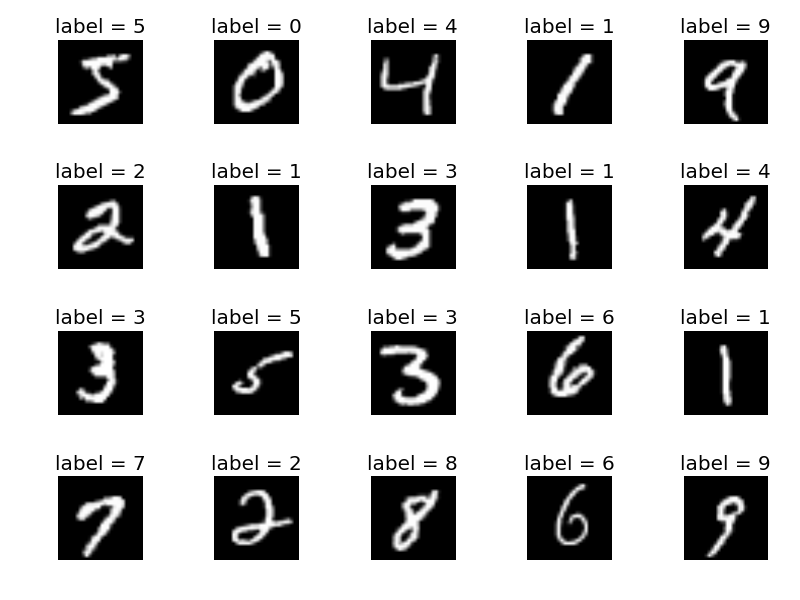
\includegraphics[width=\linewidth]{img/2_mnist.png}
        \caption{MNIST dataset}
    \end{subfigure}
    \hfill % optional; add some horizontal spacing
    \begin{subfigure}[b]{0.45\linewidth}
        \centering
        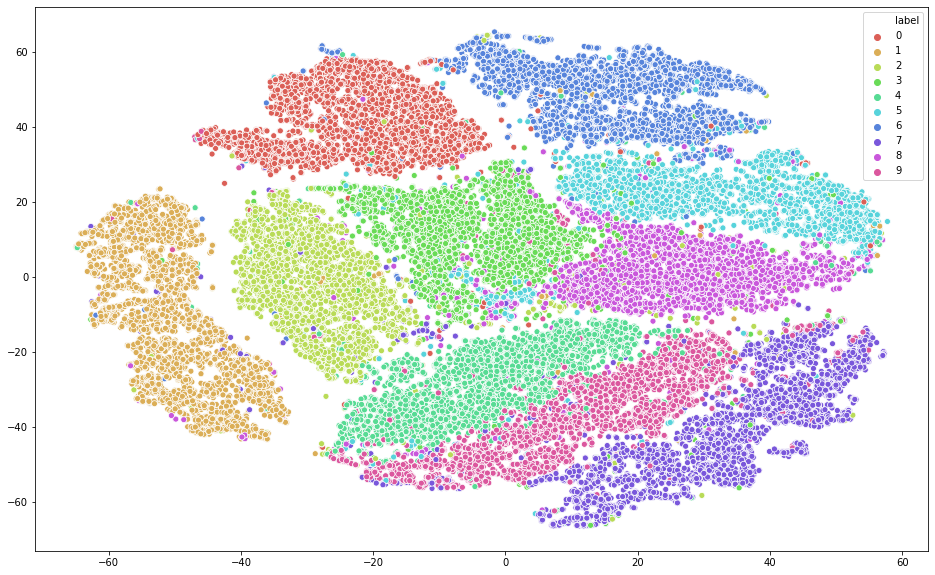
\includegraphics[width=\linewidth]{img/2_mnist-tsne.png}
        \caption{t-SNE visualisation on MNIST dataset}
        \label{fig:mnist-tsne}
    \end{subfigure}
    \caption{{\footnotesize MNIST dataset (dimension 10) and its corresponding t-SNE visualisation}}
    \label{fig:mnist-tsne}
\end{figure}




\end{enumerate}


\section{Supervised Learning}
Supervised learning assumes that we have access to input-output pairs of datapoints, $(\bm{x}, \bm{y})$, with $\bm{x} \in \mathbb{R}^n$ and $\bm{y} \in \mathbb{R}^m$, forming our dataset\sidenote{The slides replaced $K$ with $N$. Notation!} $\{(\bm{x}^{(i)}, \bm{y}^{(i)})\}_{i=1}^N$. 


\section{Linear Regression Model}
Assuming a domain of $\mathbb{R}^n$ and a one-dimensional co-domain, we can write our model as $f(\bm{x}) = \bm{x}^\top \bm{\theta}$. Thus we have:




\[
\hat{y}^{(i)} = \bm{x}^{(i)\top} \bm{\theta}
\]

The goal of learning is to find $\bm{\theta}$ such that $\hat{y}^{(i)} \approx y^{(i)}$. \marginnote{You may recall linear models written as affine transformations: $y = mx + b$, where $b$ is the bias or constant term – this makes the model affine and not linear. Linear models refers to the relationship between model parameters and predictions via a linear transformation.
}



\defb{Linear Transformation}{
A linear transformation between two vector spaces $V$ and $W$ is a map 

$$T : V \rightarrow W$$

such that:

\begin{itemize}
    \item $T(v_1 + v_2) = T(v_1) + T(v_2) \quad \forall v_1, v_2 \in V$
    \item $T(\alpha v) = \alpha T(v) \quad \forall v \in V \text{ and scalar }\alpha $
\end{itemize}

}

\marginnote[-70pt]{
    \defsb{Affine Transformations}{
        Affine transformations are more general than linear transformations, because they include not only scaling and rotation, but also translations.
    }
}


Now we are faced with something interesting: $T(\mb{0}) = \mb{0}$. According to our affine transformation $f(x) = mx+b $ where $m,b \in \mathbb{R}$, we have $f(0x) = b \neq 0f(x)$, which doesn't allow us to have a bias term $b$. This is easily fixed with a straightforward modification to capture the affine transformation $f(x) = mx + b$: we just add a feature to the input vector $x$ that is always equal to 1, then the corresponding weight for this feature becomes the bias. Introduce:

\begin{equation}
    \phi(x) : \mathbf{R} \Rightarrow \mathbf{R}^2 \quad \text{such that } \phi(x) = \begin{bmatrix} 1 \\ x \end{bmatrix} 
\end{equation}

\noindent We then need parameter vector $\theta = \begin{bmatrix} b \\ m \end{bmatrix}$. 

\noindent We then have the model 
\begin{equation}
    \hat{y} = \phi(x)^\top \theta \Rightarrow \begin{bmatrix} 1 & x \end{bmatrix}  \begin{bmatrix} b \\ m \end{bmatrix} = b + mx
\end{equation}

\section{Basis Expansion}
As seen in the previous section, a model that was once restricted to lines through the origin ahs been expanded to fit the affine transformation with the aid of Basis Expansion. We can also more generally utilise it to model non-linear relationships.

\bigskip

The key idea of basis expansion is to expand a one-dimensional feature into many dimensions, and use non-linear functions to increase the expressiveness of the model.

\subsection{Example Polynomial Basis Expansion}
A one dimensional domain $x \in \mathbb{R}$ and a one dimensional co-domain $y \in \mathbb{R}$ is assumed. Our model is $\hat{y} = \phi(x)^\top \theta$. \bigskip


We choose the basis:

\begin{equation}
    \phi(x) = \begin{bmatrix} 1 \\ x \\ x^2 \end{bmatrix} \quad \phi(x) : \R^1 \rightarrow \R^3
\end{equation}

and weights:

\begin{equation}
    \theta \in \mathbb{R}^3
\end{equation}

We finally have the fully expanded function\marginnote{We use the dot product instead of transposing, for clarity of notation.}:

\begin{equation}
    \hat{y} = \begin{bmatrix} 1 \\ x \\ x^2 \end{bmatrix} \cdot \begin{bmatrix} \theta_0 \\ \theta_1 \\ \theta_2 \end{bmatrix} = \theta_0 + \theta_1 x + \theta_2 x^2
\end{equation}

This example model is a quadratic polynomial. 

\subsection{Another Example Polynomial Basis Expansion}
Again, given our model is $\hat{y} = \phi(\mb{x})^\top \theta$ where $y \in \R $ and $\mb{x} \in \R^2$. We can use the basis

\begin{equation} 
    \phi(\mb{x}) \Rightarrow \phi\left(\begin{bmatrix} x_1 \\ x_2 \end{bmatrix}\right) = \begin{bmatrix} 1 \\ x_1 \\ x_2 \\ x_1x_2 \\ x_1^2 \\ x_2^2 \end{bmatrix} \quad \phi(x) : \mbb{R}^2 \rightarrow \mbb{R}^6
\end{equation}

and with a new set of corresponding weights, we have:

\begin{equation}
    \hat{y} = \begin{bmatrix} 1 \\ x_1 \\ x_2 \\ x_1x_2 \\ x_1^2 \\ x_2^2 \end{bmatrix} \cdot  \begin{bmatrix} \theta_0 \\ \theta_1 \\ \theta_2 \\ \theta_3 \\ \theta_4 \\ \theta_5 \end{bmatrix} = \theta_0 + \theta_1 x_1 + \theta_2 x_2 + \theta_3 x_1x_2 + \theta_4 x_1^2 + \theta_5 x_2^2 \quad \theta \in \mathbb{R}^6
\end{equation}

\section{Radial Basis Function Kernel}

Polynomial basis expansion is just a single flabour of basis expansion. Another widely-used form of basis is the kernel basis expansion. One popular example is the radial basis function kernel (RBF kernel), which is a generalisation of the polynomial basis expansion. \bigskip

It takes in a fixed parameter $\gamma > 0$, defined as 

\begin{equation}
    \kappa(x, x') = \exp(-\gamma ||x - x'||^2)
\end{equation}

where $||x - x'||^2$ is the squared Euclidean distance (or more appropriately, the $L_2$ Norm) between $x$ and $x'$. In practice, one picks fixed centres $x$ and the basis expansion computes the expanded feature set w.r.t the distance to these centres.\sidenote[][-130pt]{There is more nuance to this: you may have noticed that kernel functions take in two points, unlike the polynomial basis expansion $\phi$ taking in a single point. This is because for each of the $n$ points, we compute pairwise similarities with a point's other points, and then construct a feature vector for each point, where each point $x$ is transformed into a $n$-dimensional feature vector where each dimension represents the similarity between $x$ and one of the $n$ points.  \bigskip

For example, given a dataset with three points $x_1, x_2, x_3$, and a radial basis function $\kappa(x, x')$, the RBF kernel matrix might look like this:

\begin{equation*}
    K = \begin{bmatrix} \kappa(x_1, x_1) & \kappa(x_1, x_2) & \kappa(x_1, x_3) \\ \kappa(x_2, x_1) & \kappa(x_2, x_2) & \kappa(x_2, x_3) \\ \kappa(x_3, x_1) & \kappa(x_3, x_2) & \kappa(x_3, x_3) \end{bmatrix}
\end{equation*}

\noindent where the feature vector for $x_1$ as an example would be 
\[\begin{bmatrix} \kappa(x_1, x_1) & \kappa(x_1, x_2) & \kappa(x_1, x_3) \end{bmatrix}\]

\noindent This is related to the use of the \href{https://medium.com/@zxr.nju/what-is-the-kernel-trick-why-is-it-important-98a98db0961d}{kernel trick.}

}

\bigskip

\begin{itemize}
    \item It is easy to see that the kernel basis expansion $\kappa(x, x')$ has a minimum value of 0. It takes a maximum value of 1 when $x = x'$ . 
    \item When two points $x$ and $x'$ are far apart, the kernel value is closer to 0, and when they are closer together, the kernel value is closer to 1. 

    \item It is quite akin to a simiarity score, and that a smaller value of $\gamma$ leads to larger similarity scores (see Figure \ref{fig:rbf_kernel}).
    
    \item It is also symmetric, $\kappa(x, x') = \kappa(x', x)$, and is always positive. 
\end{itemize}

\bigskip
\begin{figure}[h]
    \centering
    \begin{tikzpicture}
    \begin{axis}[
        width=12cm,
        height=8cm,
        xlabel={$\|x - x'\|$},
        ylabel={$K(X_1, X_2)$},
        grid=major,
        domain=-10:10,
        samples=100,
        xtick={-10,-8,...,10},
        ytick={0,0.2,...,1},
        enlargelimits=false,
        legend pos=outer north east,
        axis lines=middle,
        xlabel style={at={(axis description cs:1.15,0.05)},anchor=north},
        ylabel style={at={(axis description cs:0.05,1)},anchor=south},
        title={RBF Kernel for $\kappa = 1/2$, graph of $\exp(-x^2/2)$},
        ymin=0, ymax=1,
        xmin=-10, xmax=10
    ]
        \addplot [
            blue,
            thick,
            domain=-10:10,
        ]
        {exp(-x^2/2)};
        
        % Highlight regions
        \draw [fill=blue, opacity=0.1] (axis cs:-10,0) rectangle (axis cs:-4,1);
        \draw [fill=blue, opacity=0.1] (axis cs:4,0) rectangle (axis cs:10,1);
        
        % Add region labels
        \node at (axis cs:-7,0.1) [anchor=north] {Dissimilar};
        \node at (axis cs:7,0.1) [anchor=north] {Dissimilar};
        \node at (axis cs:0,0.1) [anchor=north] {Similar};
    
    \end{axis}
    \end{tikzpicture}
    \caption{RBF Kernel for $\kappa = 1/2$, graph of $\exp(-x^2/2)$. Areas of dissimilarity are noted when the kernel values are negligible.}
    \label{fig:rbf_kernel}
    \end{figure}
    
    The RBF kernel is actually a special case of the polynomial basis expansion, where 


\subsection{Example Radial Basis Function Kernel}
Given a one-dimensional domain and a one-dimensional co-domain, we have the model $\hat{y} = \phi(x)^\top \theta$.

\begin{equation}
    \phi(x) = \exp(-\gamma ||x - x'||^2) \quad \phi(x) : \mathbb{R}^1 \rightarrow \mathbb{R}^1
\end{equation}

and with a new set of corresponding weights, we have:

\begin{equation}
    \hat{y} = \exp(-\gamma ||x - x'||^2) \cdot \begin{bmatrix} \theta_0 \\ \theta_1 \end{bmatrix} = \theta_0 \exp(-\gamma ||x - x'||^2) + \theta_1
\end{equation}


\section{Linear Algebra}










\chapter{Blah}


\newthought{The front matter} of a book refers to all of the material that
comes before the main text.  The following table from shows a list of
material that appears in the front matter of \VDQI, \EI, \VE, and \BE
along with its page number.  Page numbers that appear in parentheses refer
to folios that do not have a printed page number (but they are still
counted in the page number sequence).

\bigskip
\begin{minipage}{\textwidth}
  \begin{center}
    \begin{tabular}{lcccc}
      \toprule
                            & \multicolumn{4}{c}{Books}                                     \\
      \cmidrule(l){2-5}
      Page content          & \vdqi                     & \ei       & \ve       & \be       \\
      \midrule
      Blank half title page & \hangp{1}                 & \hangp{1} & \hangp{1} & \hangp{1} \\
      Frontispiece\footnotemark{}
                            & \hangp{2}                 & \hangp{2} & \hangp{2} & \hangp{2} \\
      Full title page       & \hangp{3}                 & \hangp{3} & \hangp{3} & \hangp{3} \\
      Copyright page        & \hangp{4}                 & \hangp{4} & \hangp{4} & \hangp{4} \\
      Contents              & \hangp{5}                 & \hangp{5} & \hangp{5} & \hangp{5} \\
      %Blank & -- & \hangp{6} & \hangp{6} & \hangp{6} \\
      Dedication            & \hangp{6}                 & \hangp{7} & \hangp{7} & 7         \\
      %Blank & -- & \hangp{8} & -- & \hangp{8} \\
      Epigraph              & --                        & --        & \hangp{8} & --        \\
      Introduction          & \hangp{7}                 & \hangp{9} & \hangp{9} & 9         \\
      \bottomrule
    \end{tabular}
  \end{center}
\end{minipage}
\vspace{-7\baselineskip}\footnotetext{The contents of this page vary from book to book.  In
  \vdqi this page is blank; in \ei and \ve this page holds a frontispiece;
  and in \be this page contains three epigraphs.}
\vspace{7\baselineskip}

\bigskip
The design of the front matter in Tufte's books varies slightly from the
traditional design of front matter.  First, the pages in front matter are
traditionally numbered with lowercase roman numerals (\eg, i, ii, iii,
iv,~\ldots).  Second, the front matter page numbering sequence is usually
separate from the main matter page numbering.  That is, the page numbers
restart at 1 when the main matter begins.  In contrast, Tufte has
enumerated his pages with arabic numerals that share the same page counting
sequence as the main matter.

\vspace{-7\baselineskip}\marginnote{
  \extrasb{On the side note of...}{yeah}

}
\vspace{7\baselineskip}

There are also some variations in design across Tufte's four books.  The
page opposite the full title page (labeled ``frontispiece'' in the above
table) has different content in each of the books.  In \VDQI, this page is
blank; in \EI and \VE, this page holds a frontispiece; and in \BE, this
page contains three epigraphs.

The dedication appears on page~6 in \vdqi (opposite the introduction), and
is placed on its own spread in the other books.  In \ve, an epigraph shares
the spread with the opening page of the introduction.

None of the page numbers (folios) of the front matter are expressed except in
\be, where the folios start to appear on the dedication page.

\newthought{The full title page} of each of the books varies slightly in
design.  In all the books, the author's name appears at the top of the
page, the title it set just above the center line, and the publisher is
printed along the bottom margin.  Some of the differences are outlined in
the following table.

\bigskip
\begin{center}
  \footnotesize
  \begin{tabular}{lllll}
    \toprule
    Feature        & \vdqi         & \ei     & \ve     & \be           \\
    \midrule
    Author         &               &         &         &               \\
    \quad Typeface & serif         & serif   & serif   & sans serif    \\
    \quad Style    & italics       & italics & italics & upright, caps \\
    \quad Size     & 24 pt         & 20 pt   & 20 pt   & 20 pt         \\
    \addlinespace
    Title          &               &         &         &               \\
    \quad Typeface & serif         & serif   & serif   & sans serif    \\
    \quad Style    & upright       & italics & upright & upright, caps \\
    \quad Size     & 36 pt         & 48 pt   & 48 pt   & 36 pt         \\
    \addlinespace
    Subtitle       &               &         &         &               \\
    \quad Typeface & \na           & \na     & serif   & \na           \\
    \quad Style    & \na           & \na     & upright & \na           \\
    \quad Size     & \na           & \na     & 20 pt   & \na           \\
    \addlinespace
    Edition        &               &         &         &               \\
    \quad Typeface & sans serif    & \na     & \na     & \na           \\
    \quad Style    & upright, caps & \na     & \na     & \na           \\
    \quad Size     & 14 pt         & \na     & \na     & \na           \\
    \addlinespace
    Publisher      &               &         &         &               \\
    \quad Typeface & serif         & serif   & serif   & sans serif    \\
    \quad Style    & italics       & italics & italics & upright, caps \\
    \quad Size     & 14 pt         & 14 pt   & 14 pt   & 14 pt         \\
    \bottomrule
  \end{tabular}
\end{center}



\newthought{The tables of contents} in Tufte's books give us our first
glimpse of the structure of the main matter.  \VDQI is split into two
parts, each containing some number of chapters.  His other three books only
contain chapters---they're not broken into parts.




\section{Typefaces}\label{sec:typefaces1}\index{typefaces}
\index{fonts|see{typefaces}}

Tufte's books primarily use two typefaces: Bembo and Gill Sans.  Bembo is used
for the headings and body text, while Gill Sans is used for the title page and
opening epigraphs in \BE.

Since neither Bembo nor Gill Sans are available in default \LaTeX{}
installations, the \TL document classes default to using Palatino and
Helvetica, respectively.  In addition, the Bera Mono typeface is used for
\texttt{monospaced} type.

The following font sizes are defined by the \TL classes:

\begin{table}[h]\index{typefaces!sizes}
  \footnotesize%
  \begin{center}
    \begin{tabular}{lccl}
      \toprule
      \LaTeX{} size        & Font size & Leading & Used for                                             \\
      \midrule
      \verb+\tiny+         & 5         & 6       & sidenote numbers                                     \\
      \verb+\scriptsize+   & 7         & 8       & \na                                                  \\
      \verb+\footnotesize+ & 8         & 10      & sidenotes, captions                                  \\
      \verb+\small+        & 9         & 12      & quote, quotation, and verse environments             \\
      \verb+\normalsize+   & 10        & 14      & body text                                            \\
      \verb+\large+        & 11        & 15      & \textsc{b}-heads                                     \\
      \verb+\Large+        & 12        & 16      & \textsc{a}-heads, \textsc{toc} entries, author, date \\
      \verb+\LARGE+        & 14        & 18      & handout title                                        \\
      \verb+\huge+         & 20        & 30      & chapter heads                                        \\
      \verb+\Huge+         & 24        & 36      & part titles                                          \\
      \bottomrule
    \end{tabular}
  \end{center}
  \caption{A list of \LaTeX{} font sizes as defined by the \TL document classes.}
  \label{tab:font-sizes}
\end{table}

\section{Headings}\label{sec:headings1}\index{headings}

Tufte's books include the following heading levels: parts,
chapters,\sidenote{Parts and chapters are defined for the \texttt{tufte-book}
  class only.}  sections, subsections, and paragraphs.  Not defined by default
are: sub-subsections and subparagraphs.

\begin{table}[h]
  \begin{center}
    \footnotesize%
    \begin{tabular}{lcr}
      \toprule
      Heading    & Style  & Size                 \\
      \midrule
      Part       & roman  & \measure{24}{36}{40} \\
      Chapter    & italic & \measure{20}{30}{40} \\
      Section    & italic & \measure{12}{16}{26} \\
      Subsection & italic & \measure{11}{15}{26} \\
      Paragraph  & italic & 10/14                \\
      \bottomrule
    \end{tabular}
  \end{center}
  \caption{Heading styles used in \BE.}
  \label{tab:heading-styles}
\end{table}

\paragraph{Paragraph} Paragraph headings (as shown here) are introduced by
italicized text and separated from the main paragraph by a bit of space.

\section{Environments}

The following characteristics define the various environments:


\begin{table}[h]
  \begin{center}
    \footnotesize%
    \begin{tabular}{lcl}
      \toprule
      Environment & Font size            & Notes                                                 \\
      \midrule
      Body text   & \measure{10}{14}{26} &                                                       \\
      Block quote & \measure{9}{12}{24}  & Block indent (left and right) by \unit[1]{pc}         \\
      Sidenotes   & \measure{8}{10}{12}  & Sidenote number is set inline, followed by word space \\
      Captions    & \measure{8}{10}{12}  &                                                       \\
      \bottomrule
    \end{tabular}
  \end{center}
  \caption{Environment styles used in \BE.}
  \label{tab:environment-styles}
\end{table}



\begin{table}
  \centering
  \footnotesize
  \caption{Example table with limited column widths}
  \begin{tabular}{p{3cm}p{3cm}p{3cm}}
    \toprule
    \textbf{Column 1} & \textbf{Column 2} & \textbf{Column 3} \\
    \midrule
    \lipsum[1][1-3]   & \lipsum[1][1-3]   & \lipsum[1][1-3]   \\
    \midrule
    \lipsum[1][1-3]   & \lipsum[1][1-3]   & \lipsum[1][1-3]   \\
    \midrule
    \lipsum[1][1-3]   & \lipsum[1][1-3]   & \lipsum[1][1-3]   \\
    \bottomrule
  \end{tabular}
\end{table}



\chapter[On the Use of the tufte-book Document Class]{On the Use of the \texttt{tufte-book} Document Class}
\label{ch:tufte-book}

The \TL document classes define a style similar to the
style Edward Tufte uses in his books and handouts.  Tufte's style is known
for its extensive use of sidenotes, tight integration of graphics with
text, and well-set typography.  This document aims to be at once a
demonstration of the features of the \TL document classes
and a style guide to their use.

\section{Page Layout}\label{sec:page-layout}
\subsection{Headings}\label{sec:headings}\index{headings}
This style provides \textsc{a}- and \textsc{b}-heads (that is,
\Verb|\section| and \Verb|\subsection|), demonstrated above.

If you need more than two levels of section headings, you'll have to define
them yourself at the moment; there are no pre-defined styles for anything below
a \Verb|\subsection|.  As Bringhurst points out in \textit{The Elements of
  Typographic Style},\cite{Bringhurst2005} you should ``use as many levels of
headings as you need: no more, and no fewer.''

The \TL classes will emit an error if you try to use
\linebreak\Verb|\subsubsection| and smaller headings.

% let's start a new thought -- a new section
\newthought{In his later books},\cite{Tufte2006} Tufte
starts each section with a bit of vertical space, a non-indented paragraph,
and sets the first few words of the sentence in \textsc{small caps}.  To
accomplish this using this style, use the \doccmddef{newthought} command:
\begin{docspec}
  \doccmd{newthought}\{In his later books\}, Tufte starts\ldots
\end{docspec}


\section{Sidenotes}\label{sec:sidenotes}
One of the most prominent and distinctive features of this style is the
extensive use of sidenotes.  There is a wide margin to provide ample room
for sidenotes and small figures.  Any \doccmd{footnote}s will automatically
be converted to sidenotes.\footnote{This is a sidenote that was entered
  using the \texttt{\textbackslash footnote} command.}  If you'd like to place ancillary
information in the margin without the sidenote mark (the superscript
number), you can use the \doccmd{marginnote} command.\marginnote{This is a
  margin note.  Notice that there isn't a number preceding the note, and
  there is no number in the main text where this note was written.}

The specification of the \doccmddef{sidenote} command is:
\begin{docspec}
  \doccmd{sidenote}[\docopt{number}][\docopt{offset}]\{\docarg{Sidenote text.}\}
\end{docspec}

Both the \docopt{number} and \docopt{offset} arguments are optional.  If you
provide a \docopt{number} argument, then that number will be used as the
sidenote number.  It will change of the number of the current sidenote only and
will not affect the numbering sequence of subsequent sidenotes.

Sometimes a sidenote may run over the top of other text or graphics in the
margin space.  If this happens, you can adjust the vertical position of the
sidenote by providing a dimension in the \docopt{offset} argument.  Some
examples of valid dimensions are:
\begin{docspec}
  \ttfamily 1.0in \qquad 2.54cm \qquad 254mm \qquad 6\Verb|\baselineskip|
\end{docspec}
If the dimension is positive it will push the sidenote down the page; if the
dimension is negative, it will move the sidenote up the page.

While both the \docopt{number} and \docopt{offset} arguments are optional, they
must be provided in order.  To adjust the vertical position of the sidenote
while leaving the sidenote number alone, use the following syntax:
\begin{docspec}
  \doccmd{sidenote}[][\docopt{offset}]\{\docarg{Sidenote text.}\}
\end{docspec}
The empty brackets tell the \Verb|\sidenote| command to use the default
sidenote number.

If you \emph{only} want to change the sidenote number, however, you may
completely omit the \docopt{offset} argument:
\begin{docspec}
  \doccmd{sidenote}[\docopt{number}]\{\docarg{Sidenote text.}\}
\end{docspec}

The \doccmddef{marginnote} command has a similar \docarg{offset} argument:
\begin{docspec}
  \doccmd{marginnote}[\docopt{offset}]\{\docarg{Margin note text.}\}
\end{docspec}

\section{References}
References are placed alongside their citations as sidenotes,
as well.  This can be accomplished using the normal \doccmddef{cite}
command.\sidenote{The first paragraph of this document includes a citation.}

The complete list of references may also be printed automatically by using
the \doccmddef{bibliography} command.  (See the end of this document for an
example.)  If you do not want to print a bibliography at the end of your
document, use the \doccmddef{nobibliography} command in its place.

To enter multiple citations at one location,\cite[-3\baselineskip]{Tufte2006,Tufte1990} you can
provide a list of keys separated by commas and the same optional vertical
offset argument: \\
\Verb|\cite{Tufte2006,Tufte1990}|.
\begin{docspec}
  \doccmd{cite}[\docopt{offset}]\{\docarg{bibkey1,bibkey2,\ldots}\}
\end{docspec}

\section{Figures and Tables}\label{sec:figures-and-tables}
Images and graphics play an integral role in Tufte's work.
In addition to the standard \docenvdef{figure} and \docenvdef{tabular} environments,
this style provides special figure and table environments for full-width
floats.

Full page--width figures and tables may be placed in \docenvdef{figure*} or
\docenvdef{table*} environments.  To place figures or tables in the margin,
use the \docenvdef{marginfigure} or \docenvdef{margintable} environments as follows
(see figure~\ref{fig:marginfig}):

\vspace{-7\baselineskip}
\begin{marginfigure}%

  \caption{This is a margin figure.  The helix is defined by
  $x = \cos(2\pi z)$, $y = \sin(2\pi z)$, and $z = [0, 2.7]$.  The figure was
  drawn using Asymptote (\protect\url{http://asymptote.sf.net/}).}
  \label{fig:marginfig}
\end{marginfigure}
\vspace{7\baselineskip}

\begin{docspec}
  \textbackslash begin\{marginfigure\}\\
  \qquad\textbackslash includegraphics\{helix\}\\
  \qquad\textbackslash caption\{This is a margin figure.\}\\
  \qquad\textbackslash label\{fig:marginfig\}\\
  \textbackslash end\{marginfigure\}\\
\end{docspec}

The \docenv{marginfigure} and \docenv{margintable} environments accept an optional parameter \docopt{offset} that adjusts the vertical position of the figure or table.  See the ``\nameref{sec:sidenotes}'' section above for examples.  The specifications are:
\begin{docspec}
  \textbackslash{begin\{marginfigure\}[\docopt{offset}]}\\
  \qquad\ldots\\
  \textbackslash{end\{marginfigure\}}\\
  \mbox{}\\
  \textbackslash{begin\{margintable\}[\docopt{offset}]}\\
  \qquad\ldots\\
  \textbackslash{end\{margintable\}}\\
\end{docspec}

Figure~\ref{fig:fullfig} is an example of the \docenv{figure*}
environment and figure~\ref{fig:textfig} is an example of the normal
\docenv{figure} environment.




As with sidenotes and marginnotes, a caption may sometimes require vertical
adjustment. The \doccmddef{caption} command now takes a second optional
argument that enables you to do this by providing a dimension \docopt{offset}.
You may specify the caption in any one of the following forms:
\begin{docspec}
  \doccmd{caption}\{\docarg{long caption}\}\\
  \doccmd{caption}[\docarg{short caption}]\{\docarg{long caption}\}\\
  \doccmd{caption}[][\docopt{offset}]\{\docarg{long caption}\}\\
  \doccmd{caption}[\docarg{short caption}][\docopt{offset}]%
  \{\docarg{long caption}\}
\end{docspec}
A positive \docopt{offset} will push the caption down the page. The short
caption, if provided, is what appears in the list of figures/tables, otherwise
the ``long'' caption appears there. Note that although the arguments
\docopt{short caption} and \docopt{offset} are both optional, they must be
provided in order. Thus, to specify an \docopt{offset} without specifying a
\docopt{short caption}, you must include the first set of empty brackets
\Verb|[]|, which tell \doccmd{caption} to use the default ``long'' caption. As
an example, the caption to figure~\ref{fig:textfig} above was given in the form
\begin{docspec}
  \doccmd{caption}[Hilbert curves...][6pt]\{Hilbert curves...\}
\end{docspec}

Table~\ref{tab:normaltab} shows table created with the \docpkg{booktabs}
package.  Notice the lack of vertical rules---they serve only to clutter
the table's data.

\begin{table}[ht]
  \centering
  % \fontfamily{ppl}\selectfont
  \begin{tabular}{ll}
    \toprule
    Margin                    & Length                          \\
    \midrule
    Paper width               & \unit[8\nicefrac{1}{2}]{inches} \\
    Paper height              & \unit[11]{inches}               \\
    Textblock width           & \unit[6\nicefrac{1}{2}]{inches} \\
    Textblock/sidenote gutter & \unit[\nicefrac{3}{8}]{inches}  \\
    Sidenote width            & \unit[2]{inches}                \\
    \bottomrule
  \end{tabular}
  \caption{Here are the dimensions of the various margins used in the Tufte-handout class.}
  \label{tab:normaltab}
  %\zsavepos{pos:normaltab}
\end{table}

\newthought{Occasionally} \LaTeX{} will generate an error message:\label{err:too-many-floats}
\begin{docspec}
  Error: Too many unprocessed floats
\end{docspec}
\LaTeX{} tries to place floats in the best position on the page.  Until it's
finished composing the page, however, it won't know where those positions are.
If you have a lot of floats on a page (including sidenotes, margin notes,
figures, tables, etc.), \LaTeX{} may run out of ``slots'' to keep track of them
and will generate the above error.

\LaTeX{} initially allocates 18 slots for storing floats.  To work around this
limitation, the \TL document classes provide a \doccmddef{morefloats} command
that will reserve more slots.

The first time \doccmd{morefloats} is called, it allocates an additional 34
slots.  The second time \doccmd{morefloats} is called, it allocates another 26
slots.

The \doccmd{morefloats} command may only be used two times.  Calling it a
third time will generate an error message.  (This is because we can't safely
allocate many more floats or \LaTeX{} will run out of memory.)

If, after using the \doccmd{morefloats} command twice, you continue to get the
\texttt{Too many unprocessed floats} error, there are a couple things you can
do.

The \doccmddef{FloatBarrier} command will immediately process all the floats
before typesetting more material.  Since \doccmd{FloatBarrier} will start a new
paragraph, you should place this command at the beginning or end of a
paragraph.

The \doccmddef{clearpage} command will also process the floats before
continuing, but instead of starting a new paragraph, it will start a new page.

You can also try moving your floats around a bit: move a figure or table to the
next page or reduce the number of sidenotes.  (Each sidenote actually uses
\emph{two} slots.)

After the floats have placed, \LaTeX{} will mark those slots as unused so they
are available for the next page to be composed.

\section{Captions}
You may notice that the captions are sometimes misaligned.
Due to the way \LaTeX's float mechanism works, we can't know for sure where it
decided to put a float. Therefore, the \TL document classes provide commands to
override the caption position.

\paragraph{Vertical alignment} To override the vertical alignment, use the
\doccmd{setfloatalignment} command inside the float environment.  For
example:

\begin{fullwidth}
  \begin{docspec}
    \textbackslash begin\{figure\}[btp]\\
    \qquad \textbackslash includegraphics\{sinewave\}\\
    \qquad \textbackslash caption\{This is an example of a sine wave.\}\\
    \qquad \textbackslash label\{fig:sinewave\}\\
    \qquad \hlred{\textbackslash setfloatalignment\{b\}\% forces caption to be bottom-aligned}\\
    \textbackslash end\{figure\}
  \end{docspec}
\end{fullwidth}

\noindent The syntax of the \doccmddef{setfloatalignment} command is:

\begin{docspec}
  \doccmd{setfloatalignment}\{\docopt{pos}\}
\end{docspec}

\noindent where \docopt{pos} can be either \texttt{b} for bottom-aligned
captions, or \texttt{t} for top-aligned captions.

\paragraph{Horizontal alignment}\label{par:overriding-horizontal}
To override the horizontal alignment, use either the \doccmd{forceversofloat}
or the \doccmd{forcerectofloat} command inside of the float environment.  For
example:

\begin{fullwidth}
  \begin{docspec}
    \textbackslash begin\{figure\}[btp]\\
    \qquad \textbackslash includegraphics\{sinewave\}\\
    \qquad \textbackslash caption\{This is an example of a sine wave.\}\\
    \qquad \textbackslash label\{fig:sinewave\}\\
    \qquad \hlred{\textbackslash forceversofloat\% forces caption to be set to the left of the float}\\
    \textbackslash end\{figure\}
  \end{docspec}
\end{fullwidth}

The \doccmddef{forceversofloat} command causes the algorithm to assume the
float has been placed on a verso page---that is, a page on the left side of a
two-page spread.  Conversely, the \doccmddef{forcerectofloat} command causes
the algorithm to assume the float has been placed on a recto page---that is, a
page on the right side of a two-page spread.


\section{Full-width text blocks}

In addition to the new float types, there is a \docenvdef{fullwidth}
environment that stretches across the main text block and the sidenotes
area.

\begin{Verbatim}
  \begin{fullwidth}
    Lorem ipsum dolor sit amet...
  \end{fullwidth}
\end{Verbatim}

\begin{fullwidth}
  \small\itshape\lipsum[1]
\end{fullwidth}

\section{Typography}\label{sec:typography}

\subsection{Typefaces}\label{sec:typefaces}\index{typefaces}
If the Palatino, \textsf{Helvetica}, and \texttt{Bera Mono} typefaces are installed, this style
will use them automatically.  Otherwise, we'll fall back on the Computer Modern
typefaces.

\subsection{Letterspacing}\label{sec:letterspacing}
This document class includes two new commands and some improvements on
existing commands for letterspacing.

When setting strings of \allcaps{ALL CAPS} or \smallcaps{small caps}, the
letter\-spacing---that is, the spacing between the letters---should be
increased slightly.\cite[][p.32]{Bringhurst2005} The \doccmddef{allcaps} command has proper letterspacing for
strings of \allcaps{FULL CAPITAL LETTERS}, and the \doccmddef{smallcaps} command
has letterspacing for \smallcaps{small capital letters}.  These commands
will also automatically convert the case of the text to upper- or
lowercase, respectively.

The \doccmddef{textsc} command has also been redefined to include
letterspacing.  The case of the \doccmd{textsc} argument is left as is,
however.  This allows one to use both uppercase and lowercase letters:
\textsc{The Initial Letters Of The Words In This Sentence Are Capitalized.}



\section{Document Class Options}\label{sec:options}

\index{class options|(}
The \doccls{tufte-book} class is based on the \LaTeX\ \doccls{book}
document class.  Therefore, you can pass any of the typical book
options.  There are a few options that are specific to the
\doccls{tufte-book} document class, however.

The \docclsoptdef{a4paper} option will set the paper size to \smallcaps{A4} instead of
the default \smallcaps{US} letter size.

The \docclsoptdef{sfsidenotes} option will set the sidenotes and title block in a
\textsf{sans serif} typeface instead of the default roman.

The \docclsoptdef{twoside} option will modify the running heads so that the page
number is printed on the outside edge (as opposed to always printing the page
number on the right-side edge in \docclsoptdef{oneside} mode).

The \docclsoptdef{symmetric} option typesets the sidenotes on the outside edge of
the page.  This is how books are traditionally printed, but is contrary to
Tufte's book design which sets the sidenotes on the right side of the page.
This option implicitly sets the \docclsopt{twoside} option.

The \docclsoptdef{justified} option sets alldocclsoptdef
and right).  The default is to set the text ragged right.
The body text of Tufte's books are set ragged right.  This prevents
needless hyphenation and makes it easier to read the text in the slightly
narrower column.

The \docclsoptdef{bidi} option loads the \docpkg{bidi} package which is used with
\tXeLaTeX\ to typeset bi-directional text.  Since the \docpkg{bidi}
package needs to be loaded before the sidenotes and cite commands are defined,
it can't be loaded in the document preamble.

The \docclsoptdef{debug} option causes the \TL classes to output debug
information to the log file which is useful in troubleshooting bugs.  It will
also cause the graphics to be replaced by outlines.

The \docclsoptdef{nofonts} option prevents the \TL classes from
automatically loading the Palatino and Helvetica typefaces.  You should use
this option if you wish to load your own fonts.  If you're using \tXeLaTeX, this
option is implied (\ie, the Palatino and Helvetica fonts aren't loaded if you
use \tXeLaTeX).

The \docclsoptdef{nols} option inhibits the letterspacing code.  The \TL\
classes try to load the appropriate letterspacing package (either pdf\TeX's
\docpkg{letterspace} package or the \docpkg{soul} package).  If you're using
\tXeLaTeX\ with \docpkg{fontenc}, however, you should configure your own
letterspacing.

The \docclsoptdef{notitlepage} option causes \doccmd{maketitle} to generate a title
block instead of a title page.  The \doccls{book} class defaults to a title
page and the \doccls{handout} class defaults to the title block.  There is an
analogous \docclsoptdef{titlepage} option that forces \doccmd{maketitle} to
generate a full title page instead of the title block.

The \docclsoptdef{notoc} option suppresses \TL's custom table of contents
(\textsc{toc}) design.  The current \textsc{toc} design only shows unnumbered
chapter titles; it doesn't show sections or subsections.  The \docclsopt{notoc}
option will revert to \LaTeX's \textsc{toc} design.

The \docclsoptdef{nohyper} option prevents the \docpkg{hyperref} package from
being loaded.  The default is to load the \docpkg{hyperref} package and use the
\doccmd{title} and \doccmd{author} contents as metadata for the generated
\textsc{pdf}.

\index{class options|)}



\chapter[Customizing Tufte-LaTeX]{Customizing \TL}
\label{ch:customizing}

The \TL document classes are designed to closely emulate Tufte's book
design by default.  However, each document is different and you may encounter
situations where the default settings are insufficient.  This chapter explores
many of the ways you can adjust the \TL document classes to better fit
your needs.

\section{File Hooks}
\label{sec:filehooks}

\index{file hooks|(}
If you create many documents using the \TL classes, it's easier to
store your customizations in a separate file instead of copying them into the
preamble of each document.  The \TL classes provide three file hooks:
\docfilehook{tufte-common-local.tex}{common}, \docfilehook{tufte-book-local.tex}{book}, and
\docfilehook{tufte-handout-local.tex}{handout}.\sloppy

\begin{description}
  \item[\docfilehook{tufte-common-local.tex}{common}]
    If this file exists, it will be loaded by all of the \TL document
    classes just prior to any document-class-specific code.  If your
    customizations or code should be included in both the book and handout
    classes, use this file hook.
  \item[\docfilehook{tufte-book-local.tex}{book}]
    If this file exists, it will be loaded after all of the common and
    book-specific code has been read.  If your customizations apply only to the
    book class, use this file hook.
  \item[\docfilehook{tufte-common-handout.tex}{handout}]
    If this file exists, it will be loaded after all of the common and
    handout-specific code has been read.  If your customizations apply only to
    the handout class, use this file hook.
\end{description}

\index{file hooks|)}

\section{Numbered Section Headings}
\label{sec:numbered-sections}
\index{headings!numbered}

While Tufte dispenses with numbered headings in his books, if you require them,
they can be anabled by changing the value of the \doccounter{secnumdepth}
counter.  From the table below, select the heading level at which numbering
should stop and set the \doccounter{secnumdepth} counter to that value.  For
example, if you want parts and chapters numbered, but don't want numbering for
sections or subsections, use the command:
\begin{docspec}
  \doccmd{setcounter}\{secnumdepth\}\{0\}
\end{docspec}

The default \doccounter{secnumdepth} for the \TL document classes is $-1$.

\begin{table}
  \footnotesize
  \begin{center}
    \begin{tabular}{lr}
      \toprule
      Heading level                         & Value \\
      \midrule
      Part (in \doccls{tufte-book})         & $-1$  \\
      Part (in \doccls{tufte-handout})      & $0$   \\
      Chapter (only in \doccls{tufte-book}) & $0$   \\
      Section                               & $1$   \\
      Subsection                            & $2$   \\
      Subsubsection                         & $3$   \\
      Paragraph                             & $4$   \\
      Subparagraph                          & $5$   \\
      \bottomrule
    \end{tabular}
  \end{center}
  \caption{Heading levels used with the \texttt{secnumdepth} counter.}
\end{table}

\section{Changing the Paper Size}
\label{sec:paper-size}

The \TL classes currently only provide three paper sizes: \textsc{a4},
\textsc{b5}, and \textsc{us} letter.  To specify a different paper size (and/or
margins), use the \doccmd[geometry]{geometrysetup} command in the preamble of your
document (or one of the file hooks).  The full documentation of the
\doccmd{geometrysetup} command may be found in the \docpkg{geometry} package
documentation.\cite[-1em][p.33]{pkg-geometry}


\section{Customizing Marginal Material}
\label{sec:marginal-material}

Marginal material includes sidenotes, citations, margin notes, and captions.
Normally, the justification of the marginal material follows the justification
of the body text.  If you specify the \docclsopt{justified} document class
option, all of the margin material will be fully justified as well.  If you
don't specify the \docclsopt{justified} option, then the marginal material will
be set ragged right.

You can set the justification of the marginal material separately from the body
text using the following document class options: \docclsopt{sidenote},
\docclsopt{marginnote}, \docclsopt{caption}, \docclsopt{citation}, and
\docclsopt{marginals}.  Each option refers to its obviously corresponding
marginal material type.  The \docclsopt{marginals} option simultaneously sets
the justification on all four marginal material types.

Each of the document class options takes one of five justification types:
\begin{description}
  \item[\docclsopt{justified}] Fully justifies the text (sets it flush left and
    right).
  \item[\docclsopt{raggedleft}] Sets the text ragged left, regardless of which
    page it falls on.
  \item[\docclsopt{raggedright}] Sets the text ragged right, regardless of
    which page it falls on.
  \item[\doccls{raggedouter}] Sets the text ragged left if it falls on the
    left-hand (verso) page of the spread and otherwise sets it ragged right.
    This is useful in conjunction with the \docclsopt{symmetric} document class
    option.
  \item[\docclsopt{auto}] If the \docclsopt{justified} document class option
    was specified, then set the text fully justified; otherwise the text is set
    ragged right.  This is the default justification option if one is not
    explicitly specified.
\end{description}

\noindent For example,
\begin{docspec}
  \doccmdnoindex{documentclass}[symmetric,justified,marginals=raggedouter]\{tufte-book\}
\end{docspec}
will set the body text of the document to be fully justified and all of the
margin material (sidenotes, margin notes, captions, and citations) to be flush
against the body text with ragged outer edges.

\newthought{The font and style} of the marginal material may also be modified using the following commands:

\begin{docspec}
  \doccmd{setsidenotefont}\{\docopt{font commands}\}\\
  \doccmd{setcaptionfont}\{\docopt{font commands}\}\\
  \doccmd{setmarginnotefont}\{\docopt{font commands}\}\\
  \doccmd{setcitationfont}\{\docopt{font commands}\}
\end{docspec}

The \doccmddef{setsidenotefont} sets the font and style for sidenotes, the
\doccmddef{setcaptionfont} for captions, the \doccmddef{setmarginnotefont} for
margin notes, and the \doccmddef{setcitationfont} for citations.  The
\docopt{font commands} can contain font size changes (e.g.,
\doccmdnoindex{footnotesize}, \doccmdnoindex{Huge}, etc.), font style changes (e.g.,
\doccmdnoindex{sffamily}, \doccmdnoindex{ttfamily}, \doccmdnoindex{itshape}, etc.), color changes (e.g.,
\doccmdnoindex{color}\texttt{\{blue\}}), and many other adjustments.

If, for example, you wanted the captions to be set in italic sans serif, you could use:
\begin{docspec}
  \doccmd{setcaptionfont}\{\doccmdnoindex{itshape}\doccmdnoindex{sffamily}\}
\end{docspec}

\chapter{Compatibility Issues}
\label{ch:compatibility}

When switching an existing document from one document class to a \TL document class, a few changes to the document may have to be made.

\section{Converting from \doccls{article} to \doccls{tufte-handout}}

The following \doccls{article} class options are unsupported: \docclsopt{10pt}, \docclsopt{11pt}, \docclsopt{12pt}, \docclsopt{a5paper}, \docclsopt{b5paper}, \docclsopt{executivepaper}, \docclsopt{legalpaper}, \docclsopt{landscape}, \docclsopt{onecolumn}, and \doccls{twocolumn}.

The following headings are not supported: \doccmd{subsubsection} and \doccmd{subparagraph}.

\section{Converting from \doccls{book} to \doccls{tufte-book}}

The following \doccls{report} class options are unsupported: \docclsopt{10pt}, \docclsopt{11pt}, \docclsopt{12pt}, \docclsopt{a5paper}, \docclsopt{b5paper}, \docclsopt{executivepaper}, \docclsopt{legalpaper}, \docclsopt{landscape}, \docclsopt{onecolumn}, and \doccls{twocolumn}.

The following headings are not supported: \doccmd{subsubsection} and \doccmd{subparagraph}.



\chapter{Troubleshooting and Support}
\label{ch:troubleshooting}

\section{\TL Website}\label{sec:website}
The website for the \TL packages is located at
\url{http://code.google.com/p/tufte-latex/}.  On our website, you'll find
links to our \smallcaps{svn} repository, mailing lists, bug tracker, and documentation.

\section{\TL Mailing Lists}\label{sec:mailing-lists}
There are two mailing lists for the \TL project:

\paragraph{Discussion list}
The \texttt{tufte-latex} discussion list is for asking questions, getting
assistance with problems, and help with troubleshooting.  Release announcements
are also posted to this list.  You can subscribe to the \texttt{tufte-latex}
discussion list at \url{http://groups.google.com/group/tufte-latex}.

\paragraph{Commits list}
The \texttt{tufte-latex-commits} list is a read-only mailing list.  A message
is sent to the list any time the \TL code has been updated.  If you'd like to
keep up with the latest code developments, you may subscribe to this list.  You
can subscribe to the \texttt{tufte-latex-commits} mailing list at
\url{http://groups.google.com/group/tufte-latex-commits}.

\section{Getting Help}\label{sec:getting-help}
If you've encountered a problem with one of the \TL document classes, have a
question, or would like to report a bug, please send an email to our
mailing list or visit our website.

To help us troubleshoot the problem more quickly, please try to compile your
document using the \docclsopt{debug} class option and send the generated
\texttt{.log} file to the mailing list with a brief description of the problem.



\section{Errors, Warnings, and Informational Messages}\label{sec:tl-messages}
The following is a list of all of the errors, warnings, and other messages generated by the \TL classes and a brief description of their meanings.
\index{error messages}\index{warning messages}\index{debug messages}

% Errors
\docmsg{Error: \doccmd{subparagraph} is undefined by this class.}{%
  The \doccmd{subparagraph} command is not defined in the \TL document classes.
  If you'd like to use the \doccmd{subparagraph} command, you'll need to redefine
  it yourself.  See the ``Headings'' section on page~\pageref{sec:headings} for a
  description of the heading styles availaboe in the \TL document classes.}

\docmsg{Error: \doccmd{subsubsection} is undefined by this class.}{%
  The \doccmd{subsubsection} command is not defined in the \TL document classes.
  If you'd like to use the \doccmd{subsubsection} command, you'll need to
  redefine it yourself.  See the ``Headings'' section on
  page~\pageref{sec:headings} for a description of the heading styles availaboe
  in the \TL document classes.}

\docmsg{Error: You may only call \doccmd{morefloats} twice. See the\par\noindent\ \ \ \ \ \ \ \ Tufte-LaTeX documentation for other workarounds.}{%
  \LaTeX{} allocates 18 slots for storing floats.  The first time
  \doccmd{morefloats} is called, it allocates an additional 34 slots.  The second
  time \doccmd{morefloats} is called, it allocates another 26 slots.

  The \doccmd{morefloats} command may only be called two times.  Calling it a
  third time will generate this error message.  See
  page~\pageref{err:too-many-floats} for more information.}

% Warnings
\docmsg{Warning: Option `\docopt{class option}' is not supported -{}- ignoring option.}{%
This warning appears when you've tried to use \docopt{class option} with a \TL
document class, but \docopt{class option} isn't supported by the \TL document
class.  In this situation, \docopt{class option} is ignored.}

% Info / Debug messages
\docmsg{Info: The `\docclsopt{symmetric}' option implies `\docclsopt{twoside}'}{%
  You specified the \docclsopt{symmetric} document class option.  This option automatically forces the \docclsopt{twoside} option as well.  See page~\pageref{clsopt:symmetric} for more information on the \docclsopt{symmetric} class option.}


\section{Package Dependencies}\label{sec:dependencies}
The following is a list of packages that the \TL document
classes rely upon.  Packages marked with an asterisk are optional.
\begin{multicols}{2}
  \begin{itemize}
    \item xifthen
    \item ifpdf*
    \item ifxetex*
    \item hyperref
    \item geometry
    \item ragged2e
    \item chngpage \emph{or} changepage
    \item paralist
    \item textcase
    \item soul*
    \item letterspace*
    \item setspace
    \item natbib \emph{and} bibentry
    \item optparams
    \item placeins
    \item mathpazo*
    \item helvet*
    \item fontenc
    \item beramono*
    \item fancyhdr
    \item xcolor
    \item textcomp
    \item titlesec
    \item titletoc
  \end{itemize}
\end{multicols}




%%
% The back matter contains appendices, bibliographies, indices, glossaries, etc.







\backmatter

% \bibliography{sample-handout}
% \bibliographystyle{plainnat}


\printindex

\end{document}
